%%%%%%%%%%%%%%%%%%%%%%%%%%%%%%%%%%%%%%%%%
% Simple Sectioned Essay Template
% LaTeX Template
%
% This template has been downloaded from:
% http://www.latextemplates.com
%
%%%%%%%%%%%%%%%%%%%%%%%%%%%%%%%%%%%%%%%%%

%----------------------------------------------------------------------------------------
%	PACKAGES AND OTHER DOCUMENT CONFIGURATIONS
%----------------------------------------------------------------------------------------

\documentclass[
12pt,
ngerman,
oneside]
{scrbook} % Default font size is 12pt, it can be changed here

\usepackage[parfill]{parskip} % to avoid ident on newline

\usepackage{geometry} % Required to change the page size to A4
\geometry{a4paper,left=2.5cm, right=2.5cm, top=2.5cm, bottom=2.5cm} % Set the page size to be A4 as opposed to the default US Letter

\usepackage{graphicx} % Required for including pictures

\usepackage{float} % Allows putting an [H] in \begin{figure} to specify the exact location of the figure
\usepackage{wrapfig} % Allows in-line images such as the example fish picture

\usepackage{subfigure}

\usepackage{syntax} % ebnf

\linespread{1.15} % Line spacing

\graphicspath{{Pictures/}} % Specifies the directory where pictures are stored

\usepackage{paralist}

\usepackage{amssymb}

\usepackage[ngerman]{babel}
\usepackage[utf8]{inputenc}
\usepackage[T1]{fontenc}
\usepackage[usenames, dvipsnames]{xcolor}

\definecolor[named]{myColorMainA}{RGB}{0,26,153}
\definecolor[named]{myColorMainB}{RGB}{174,49,54}

\usepackage[pdftex]{hyperref}       
\hypersetup{
	bookmarksopen=true,
	bookmarksopenlevel=3,
	colorlinks = true,
	linkcolor  = black,
	citecolor=black
}

\usepackage{scrextend}

\usepackage[backend=bibtex,style=numeric-comp]{biblatex}
\bibliography{bib/literatur.bib}

% Nummerierungstiefen
\setcounter{tocdepth}{3} 
\setcounter{secnumdepth}{3} 		

\usepackage{csquotes}

\usepackage{scrextend}
\addtokomafont{labelinglabel}{\sffamily}
\usepackage[inline]{enumitem}

\usepackage{titlesec}
\usepackage{sectsty}
\chapterfont{\color{myColorMainA}}
\sectionfont{\color{myColorMainA}}  % sets color of sections
\subsectionfont{\color{myColorMainA}} 
\subsubsectionfont{\color{myColorMainA}} 
\paragraphfont{\color{myColorMainA}} 
\subparagraphfont{\color{myColorMainA}} 
\definecolor{gray75}{gray}{0.75}
\newcommand{\hsp}{\hspace{20pt}}
\titleformat{\chapter}[hang]{\Huge\bfseries\color{myColorMainA}}{\thechapter\hsp\textcolor{gray75}{|}\hsp}{0pt}{\Huge\bfseries}

\chapterfont{\color{myColorMainA}}

\usepackage{fancyhdr}
\setlength{\headheight}{15pt}

\pagestyle{fancy}
\renewcommand{\chaptermark}[1]{ \markboth{#1}{} }
\renewcommand{\sectionmark}[1]{ \markright{#1} }

\fancyhf{}
\fancyhead[LE,RO]{\thepage}
\fancyhead[RE]{\textit{ \nouppercase{\leftmark}} }
\fancyhead[LO]{\textit{ \nouppercase{\rightmark}} }

\fancypagestyle{plain}{ %
	\fancyhf{} % remove everything
	\renewcommand{\headrulewidth}{0pt} % remove lines as well
	\renewcommand{\footrulewidth}{0pt}
}

%% begin lstlisting --------------------------------------------
\usepackage{caption}
\usepackage{listings}
\usepackage{textcomp} % to have single quotes like this '

% Define Colors
\definecolor{rotpink}{RGB}{168,1,99}
\definecolor{lightgray}{rgb}{.9,.9,.9}
\definecolor{darkgray}{rgb}{.4,.4,.4}
\definecolor{purple}{rgb}{0.65, 0.12, 0.82}

\definecolor{eclipseBlue}{RGB}{42,0.0,255}
\definecolor{eclipseGreen}{RGB}{63,127,95}
\definecolor{eclipsePurple}{RGB}{127,0,85}

% Defines a new code listing style
\lstdefinestyle{numbered-and-boxed}{
	frame=trbl, % draw a frame at the top, right, left and bottom of the listing
	frameround=tttt, % make the frame round at all four corners
	framesep=4pt, % quarter circle size of the round corners
	numbers=left, % show line numbers at the left
	numberstyle=\tiny\ttfamily, % style of the line numbers	
	numbersep=10pt
}

\lstdefinestyle{numbered-and-lines}{
	frame=lines, % draw a frame at the top, right, left and bottom of the listing
	numbers=left, % show line numbers at the left
	numberstyle=\tiny\ttfamily, % style of the line numbers
	numbersep=10pt
}

\lstdefinestyle{only-lines}{
	frame=lines, % draw a frame at the top, right, left and bottom of the listing
}

\lstdefinestyle{only-rect}{
	frame=trbl, % draw a frame at the top, right, left and bottom of the listing
}

% Define Language
\lstdefinelanguage{javascript}{
	% list of keywords (reserved words)
	keywords={abstract, arguments, await, boolean, break, byte, case, catch, char, class, const, continue, debugger, default, delete, do, double, else, enum, eval, export, extends, false, final, finally, float, for, function, goto, if, implements, import, in, instanceof, int, interface, let, long, native, new, null, package, private, protected, public, return, short, static, super, switch, synchronized, this, throw, throws, transient, true, try, typeof, var, void, volatile, while, with, yield},
	keywordstyle=\color{eclipsePurple},
	% list of built-in objects, properties and methods, which shouldn't be used
	deletekeywords={}, % delete single first class keywords	and use them as 2. class
	morekeywords={[2]{Array, Date, eval, function, hasOwnProperty, Infinity, isFinite, isNaN, isPrototypeOf, length, Math, NaN, name, Number, Object, prototype, String, toString, undefined, valueof}},
	keywordstyle={[2]{\color{eclipseBlue}\bfseries}},
	% list of HTML and Window objects and properties, which shouldn't be used
	morekeywords={[3]{alert, all, anchor, anchors, area, assign, blur, button, checkbox, clearInterval, clearTimeout, clientInformation, close, closed, confirm, constructor, crypto, decodeURI, decodeURIComponent, defaultStatus, document, element, elements, embed, embeds, encodeURI, encodeURIComponent, escape, event, fileUpload, focus, form, forms, frame, innerHeight, innerWidth, layer, layers, link, location, mimeTypes, navigate, navigator, frames, frameRate, hidden, history, image, images, offscreenBuffering, open, opener, option, outerHeight, outerWidth, packages, pageXOffset, pageYOffset, parent, parseFloat, parseInt, password, pkcs11, plugin, prompt, propertyIsEnum, radio, reset, screenX, screenY, scroll, secure, select, self, setInterval, setTimeout, status, submit, taint, text, textarea, top, unescape, untaint, window}},
	keywordstyle={[3]{\color{eclipseBlue}\bfseries}},
	% list of HTML Event handels, which shouldn't be used as identifiers
	morekeywords={[4]{onblur, onclick, onerror, onfocus, onkeydown, onkeypress, onkeyup, onmouseover, onload, onmouseup, onmousedown, onsubmit}},
	keywordstyle={[4]{\color{eclipseBlue}\bfseries}},
	keywordstyle={[3]{\color{eclipseBlue}\bfseries}},
	% node.js built-in's, which shouldn't be used as identifiers
	morekeywords={[5]{require, module, exports}},
	keywordstyle={[5]{\color{eclipseBlue}\bfseries}},
	identifierstyle=\color{black},
	sensitive=true, % keywords are case-sensitive in JavaScript
	comment=[l]{//}, % l is for line comment
	morecomment=[s]{/*}{*/}, % s is for start and end delimiter
	commentstyle=\color{darkgray},
	stringstyle=\color{eclipseGreen},
	morestring=[m]', % defines that strings are enclosed in single quotes
	morestring=[m]", % defines that strings are enclosed in double quotes
	alsoletter=?,
	alsodigit=-
}

\lstdefinelanguage{purescript}{
	% list of keywords (reserved words)
	keywords={data, type, newtype, foreign, import, infixl, infixr, infix, class, instance, module, case, of, if, then, else, do, let, true, false, in, where, forall},
	keywordstyle=\color{eclipsePurple},
	% list of reserved operators, which shouldn't be used
	deletekeywords={}, % delete single first class keywords	and use them as 2. class
	morekeywords={[2]{=>, ->, =, ., \\\\}},
	keywordstyle={[2]{\color{black}\bfseries}},
	% built-in functions
	morekeywords={[3]{lookup}},
	keywordstyle={[3]{\color{eclipseBlue}\bfseries}},
	% built-in data types
	morekeywords={[4]{String, Map}},
	keywordstyle={[4]{\color{eclipseBlue}\bfseries}},
	identifierstyle=\color{black},
	sensitive=true, % keywords are case-sensitive in JavaScript
	comment=[l]{--}, % l is for line comment
	morecomment=[s]{\{-}{-\}}, % s is for start and end delimiter
	commentstyle=\color{darkgray},
	stringstyle=\color{eclipseGreen},
	morestring=[m]', % defines that strings are enclosed in single quotes
	morestring=[m]", % defines that strings are enclosed in double quotes
	alsoletter={=>, ->, =, ., \\\\},
	alsodigit=-
}

% Set Language, basic common setup for all javascript listings
\lstset{
	language={javascript},
	basicstyle=\small\ttfamily, % Global Code Style
	captionpos=b, % Position of the Caption (t for top, b for bottom)
	extendedchars=true, % Allows 256 instead of 128 ASCII characters
	tabsize=2, % number of spaces indented when discovering a tab 
	showtabs=false,
	columns=fixed, % make all characters equal width
	keepspaces=true, % does not ignore spaces to fit width, convert tabs to spaces
	showstringspaces=false, % lets spaces in strings appear as real spaces
	breaklines=true, % wrap lines if they don't fit
	upquote=true % single quotes should look like this '
}
%% end lstlisting ----------------------------------------------


\begin{document}
	
%----------------------------------------------------------------------------------------
%	TITLE PAGE
%----------------------------------------------------------------------------------------

\begin{titlepage}
	
	\newcommand{\HRule}{\rule{\linewidth}{0.5mm}} % Defines a new command for the horizontal lines, change thickness here
	
	\center % Center everything on the page
	
	\textsc{\LARGE Technische Hochschule Mittelhessen}\\[1.5cm] % Name of your university/college
	\textsc{\Large Kernel-Architekturen in Programmiersprachen}\\[0.5cm] % Major heading such as course name
	\textsc{\large Projektarbeit}\\[0.5cm] % Minor heading such as course title
	
	\HRule \\[0.7cm]
	{ \huge \bfseries Eine Analyse der grundlegenden Übersetzungsmechanik der Sprache PureScript}\\[0.4cm] % Title of your document
	\HRule \\[1.5cm]
	
	\begin{minipage}{0.4\textwidth}
		\begin{flushleft} \large
			\emph{Autor:}\\
			Daniel \textsc{Kreck} % Your name \\
		\end{flushleft}
	\end{minipage}
	~
	\begin{minipage}{0.4\textwidth}
		\begin{flushright} \large
			\emph{Dozent:} \\
			Prof. Dr. D. \textsc{Herzberg} % Supervisor's Name
		\end{flushright}
	\end{minipage}\\[4cm]
	
	{\large \today}\\[3cm] % Date, change the \today to a set date if you want to be precise
	
	%\includegraphics{Logo}\\[1cm] % Include a department/university logo - this will require the graphicx package
	
	\vfill % Fill the rest of the page with whitespace
	
\end{titlepage}


%----------------------------------------------------------------------------------------
%	TABLE OF CONTENTS
%----------------------------------------------------------------------------------------

\tableofcontents % Include a table of contents

\newpage % Begins the essay on a new page instead of on the same page as the table of contents 


%----------------------------------------------------------------------------------------
%	CONTENT
%----------------------------------------------------------------------------------------

\chapter{Zielsetzung und Vorgehen}
In diesem Kapitel wird die Projektaufgabe des Moduls Kernel-Architekturen in Programmiersprachen, im Fachbereich MNI der Technischen Hochschule Mittelhessen, beschrieben.

\section{Kontext}
Im Rahmen des Moduls Kernel-Architekturen in Programmiersprachen beschäftigen wir uns mit Sprachen dieser Art. Dies sind Sprachen, welche aus einem kleinen Sprachkern aufgebaut und meist funktionaler Natur sind.

Der Dozent Prof. Dr. Dominikus Herzberg entwickelte zu Lehrzwecken die Kernel-basierte konkatenative Sprache Consize in der Programmiersprache Clojure. Diese galt es zum Einstieg in das Modul in einer Sprache der eigenen Wahl zu reimplementieren. Prüfungsleistung kann es sein, Consize um weitere Sprachfunktionalitäten zu erweitern oder eine Analyse einer anderen Kernel-basierten Programmiersprache vorzunehmen. 

\section{Problem}
Als individuelle Projektaufgabe soll sich mit einer Kernel-basierten Sprache beschäftigt und ihr Übersetzungsmechanismus beschrieben werden. Das dient dem Zweck zu ergründen wie dieser aussieht und aufgebaut ist, welche Sprachkonstrukte zur Abbildung genutzt werden und damit auch zu erforschen, wie eine sich in der Praxis befindliche Kernel-basierte Sprache strukturiert ist und im Kern funktioniert. Es geht also nicht um weniger, als zu erforschen, wie gut man sich einer fremden Sprache unter einem potentiell fremden Paradigma nähern kann, wenn man den Zielcode analysiert, der auf ein bereits bekanntes Paradigma aufsetzt.

\section{Aufgabe}
Dem Problem wird mit der Programmiersprache Purescript, welche nach Javascript kompiliert, begegnet. Ziel ist es Muster in der Übersetzung von PureScript nach JavaScript zu erkennen sowie zu beschreiben und sich dadurch der Sprache PureScript zu nähern.

Der Beschreibungsprozess ist wie folgt aufgebaut. Die aufgegriffenen Spachelemente von Purescript werden erklärt und damit wird kein Wissen in der Sprache selbst vorausgesetzt, um sie zu verstehen. Im Anschluss wird die Übersetzung nach Javascript aufgezeigt und diese Abbildung beschrieben. Das hat zur Folge, dass die Kapitel thematisch aufeinander aufbauen müssen. Als erstes steht bspw. das Modulkonzept von PureScript, gefolgt von Funktionen, ohne Typdeklarationen einzuführen. Diese werden erst genutzt, wenn Typen im nächsten Kapitel eingeführt wurden. Allgemeine Begriffe oder Definitionen der Informatik, insbesondere der Softwareentwicklung, werden allerdings vorausgesetzt.

Um im Vorgehen systematisch zu sein, wird sich anhand der Gliederung des Buches \glqq PureScript by Example\grqq{} von Phil Freeman orientiert. Die größten und wichtigsten Themenblöcke bilden in dieser Ausarbeitung die Kapitel. Kleinere oder von ihrer Abbildung her uninteressantere Themenbereiche fließen entweder innerhalb eines Kapitels am Rande ein oder werden nicht betrachtet. Ein Beispiel für einen wichtigen Themenblock, der ein Kapitel aufspannt, sind Typen, untergliedert in einfache Typen, Algebraische Typen und Typklassen. Ein Beispiel für einen Themenbereich, der nur am Rande einfließt, wäre bspw. Pattern Matching.


\chapter{Module und Bezeichner}
Ein PureScript Programm ist eine Sammlung von Modulen. Module definieren Namensräume und sind wiederum eine Sammlung von Funktionen, Typen sowie Typklassen für einen bestimmten Zweck. In PureScript werden Module durch das \lstinline[language=purescript, columns=fixed]{module} Schlüsselwort beschrieben. Ein Modul kann über \lstinline[language=purescript, columns=fixed]{import} weitere Funktionalität aus anderen Modulen importieren und nutzen sowie über eine Exportliste entscheiden, welche der eigenen Funktionalität für externe Module sichtbar ist \cite{PSModules18}. Durch Listing \ref{BasicModulePS} wird dieses Konzept am einfachen Beispiel der Identitätsfunktion demonstriert. Im Gegensatz zu Haskell wird die Prelude in PureScript wie jedes andere Modul behandelt und muss damit explizit importiert werden\footnote{In diesem Fall ist der Import nicht erforderlich, da keine Funktionalitäten aus der Prelude genutzt werden - ihr Import dient einzig zur Demonstration des Importmechanismus von Modulen}. Sie definiert elementare Operationen, wie z.B. bereits die Addition oder Multiplikation, sofern es sich um die standardmäßige Prelude handelt, da dieses Konzept es ebenso ermöglicht eine eigene Prelude zu definieren \cite{PSDifferences-from-Haskell18}.

\begin{lstlisting}[language=purescript, style=numbered-and-boxed, caption=Einfache Moduldefinition mit Imports und Exports in PureScript, label=BasicModulePS]
module Main (exportedIdentity) where

import Prelude

exportedIdentity x = x
notExportedIdentity x = x 
\end{lstlisting}

Das Modul mit der Bezeichnung \emph{Main} beinhaltet zwei Funktionen - zweimal die Definition der Identitätsfunktion. Die eine wird durch die Angabe zwischen Modulbezeichnung und \lstinline[language=purescript, columns=fixed]{where} Schlüsselwort, welches einen neuen Codeblock einführt, exportiert. Die andere bleibt lediglich innerhalb des Moduls zugreifbar.
Wird keine Exportliste angegeben, werden implizit alle Bestandteile des Moduls exportiert.

In Listing \ref{BasicModuleJS} ist die Übersetzung des vorangegangenen PureScript-Beispiels abgebildet. Man erkennt durch die Direktive in der ersten Zeile, dass JavaScript im Strict Mode ausgeführt werden soll. In diesem ist es bspw. nicht möglich undeklarierte Variablen zu nutzen \cite{w3schoolsJSStrictMode18}. Für den Import und Export von Modulen wird auf die Node.js Funktionen \lstinline[language=javascript, columns=fixed]{require} und  \lstinline[language=javascript, columns=fixed]{exports} zurückgegriffen. Dies bedeutet, dass Module JavaScript Objekte werden, welche die zu exportierenden Member des Moduls kapseln \cite{NodeJSModules18}.

\begin{lstlisting}[language=javascript, style=numbered-and-boxed, caption= Übersetzung der einfachen Moduldefinition nach JavaScript, label=BasicModuleJS]
"use strict";
var Prelude = require("../Prelude");

var notExportedIdentity = function (x) { return x; };
var exportedIdentity = function (x) { return x; };

module.exports = {
	exportedIdentity: exportedIdentity
};
\end{lstlisting}

 Nach dem Übersetzungsvorgang liegt im jeweiligen Ausgabeverzeichnis ein Verzeichnis, welches den Modulnamen, hier \emph{Main}, trägt und in diesem mindestens zwei weitere Dateien - eine JavaScript-Datei (index.js) mit dem entsprechenden Zielcode und eine Datei im JSON-Format (externs.json), die Metainformationen enthält. Das übersetzte Prelude-Module befindet sich mit gleicher Struktur  ebenfalls im Ausgabeverzeichnis, was dessen Import in Listing \ref{BasicModuleJS} durch die Pfadangabe bereits andeutet.

PureScript Funktionen werden zu JavaScript Funktionen übersetzt, wobei deren ursprüngliche Bezeichnungen, sofern keine Namenskonflikte entstehen, versucht werden beizubehalten \cite[][S. 10]{Freeman17}. Nutzt man zum Beispiel reservierte Bezeichner in JavaScript als Bezeichner in PureScript werden sie durch das Voranstellen zweier Dollar Symbole maskiert. Wird eine Bezeichnung in PureScript gewählt, welcher in JavaScript unzulässig ist, wird sie durch ein einfaches Dollar Symbol maskiert. In Listing \ref{NameGenerationPS} und \ref{NameGenerationJS} sind diese beiden Fälle exemplarisch aufgeführt \cite[][S. 144]{Freeman17}.

\noindent\begin{minipage}[t]{.49\textwidth} 
	\hspace*{0pt}\begin{lstlisting}[language=purescript, style=only-rect, caption= Name Generation PS, label=NameGenerationPS]
	null = []
	example' = 100
	\end{lstlisting}
\end{minipage}% 
% 
\hfill% 
\begin{minipage}[t]{.49\textwidth} 
	\hspace*{0pt}\begin{lstlisting}[language=javascript, style=only-rect, caption= Name Generation JS, label=NameGenerationJS] 
	var $$null = [];
	var example$prime = 100;
	\end{lstlisting}
\end{minipage}
\hfill% 


\chapter{Kommentare}
In PureScript gibt es zwei Arten von Kommentaren - Zeilen- sowie Blockkommentare. Der PureScript Compiler ignoriert diese nicht wie üblich während der Übersetzung, sondern wandelt sie in ihr JavaScript-Pendant um und bettet sie in den Zielcode ein. Leerzeichen werden ebenfalls eins zu eins übernommen, wie in Listing \ref{CommentsPS} und \ref{CommentsJS} dargestellt.
\noindent\begin{minipage}[t]{.49\textwidth} 
	\hspace*{0pt}\begin{lstlisting}[language=purescript, style=only-rect, caption= Kommentare PS, label=CommentsPS]
	-- single line comment
	
	{- multiline comment which can
		continue for many lines
	-}
	\end{lstlisting}
\end{minipage}% 
% 
\hfill% 
\begin{minipage}[t]{.49\textwidth} 
	\hspace*{0pt}\begin{lstlisting}[language=javascript, style=only-rect, caption= Kommentare JS, label=CommentsJS] 
	// single line comment
	
	/**
	*  multiline comment which can
	*    continue for many lines
	*/
	\end{lstlisting}
\end{minipage}
\hfill% 
Kommentare, die mit einem Pipe-Zeichen beginnen, werden als Dokumentation gesehen und erscheinen in Tools wie Pursuit\footnote{Pursuit ist ein Webdienst, der es einem erlaubt die API Dokumentation von PurseScript nach Paketen, Modulen, Funktionen usw.  zu durchsuchen - \href{https://pursuit.purescript.org/}{https://pursuit.purescript.org/}}. Im Gegensatz zu Haskell muss bei mehreren Zeilenkommentaren untereinander, jede Zeile, die als Dokumentation dienen soll, mit dem Pipe-Zeichen beginnen \cite{PSSyntax18}.


\chapter{Funktionsdefinition und -applikation}
\label{functionDefAndApp}
Funktionen in PureScript werden auf JavaScript Funktionen abgebildet und können auf oberster Ebene eines Moduls definiert werden, indem der Funktionsbezeichner gefolgt von beliebig vielen Funktionsargumenten vor dem Gleichheitszeichen und der Funktionskörper hinter diesem geschrieben werden \cite[][S. 17]{Freeman17}. Als Beispiel diene hierzu die Funktion \emph{addTwo} in Listing \ref{FunctionPS}. Alle weiteren Ausführungen beziehen sich ebenfalls auf dieses und Listing \ref{FunctionJS} (gekürzt um Strict Mode Direktive und Exports), welches dessen Übersetzung nach JavaScript aufzeigen soll. 

\begin{lstlisting}[language=purescript, style=numbered-and-boxed, caption=Funktionen in PureScript, label=FunctionPS]
module Main where

import Prelude ((+))

addTwo a b = a + b
constant = addTwo 2 3
\end{lstlisting}

\begin{lstlisting}[language=javascript, style=numbered-and-boxed, caption= Funktionen in JavaScript, label=FunctionJS]
var Data_Semiring = require("../Data.Semiring");
var Prelude = require("../Prelude");

var addTwo = function (dictSemiring) {
	return function (a) {
		return function (b) {
			return Data_Semiring.add(dictSemiring)(a)(b);
		};
	};
};

var constant = addTwo(Data_Semiring.semiringInt)(2)(3);
\end{lstlisting}

Im Vergleich zu ihrem Gegenstück in JavaScript nehmen Funktionen in PureScript immer nur ein Argument an - wie auch in Haskell \cites[][]{PSTypes18}[][Kap. Higher order functions, Abschn. Curried functions]{Haskell11}. Unsere Funktion \emph{addTwo}, welche offensichtlich zwei Argumente anzunehmen scheint, ist ein Beispiel für eine \textbf{Curried Function}\footnote{\href{https://de.wikipedia.org/wiki/Currying}{https://de.wikipedia.org/wiki/Currying}}. Aus diesem Aspekt erschließt sich die Übersetzung nach Javascript in den Zeilen fünf bis neun und auch die schrittweise Funktionsapplikation in der letzten Zeile. 

Bleibt zu erläutern wie Operationen wie die Addition, und wie die Funktionsapplikation in JavaScript umgesetzt werden. Ersteres wird auf den Abschnitt  \glqq \ref{typesAndTypeClasses} \nameref{typesAndTypeClasses}\grqq{} vertagt, da zuvor Typen und Typklassen eingeführt werden müssen. Für jetzt reicht es aus den Zielcode rund um das Modul \emph{Data.Semiring}\footnote{ist an die Algebraische Struktur des Halbringes aus der Mathematik angelehnt - \href{https://de.wikipedia.org/wiki/Halbring_(Algebraische_Struktur)}{https://de.wikipedia.org/wiki/Halbring_(Algebraische_Struktur)}} aus dem Blickwinkel zu betrachten, dass die Addition bekannterweise eine typabhängige Operation darstellt, was zu dem zusätzlichen Zielcode führt, der die bereits erläuterte Funktionalität umschließt. In diesem Fall bezieht er sich auf den Integer-Typ, weil in der Funktionsapplikation in Zeile 6 bzw. 12 des jeweiligen Listings Ganzzahlen genutzt werden und der Compiler durch Typinferenz die passende typabhängige Übersetzung vorgenommen hat - \emph{\mbox{Data_Semiring.semiringInt}} als typgebundene Berechnungsfunktion in der Funktion \emph{addTwo}.

Die Funktionsapplikation wird in PureScript durch das einfache hintereinanderschreiben (auch Juxtaposition genannt) des Funktionsbezeichners und den Argumenten durchgeführt \cite{PSSyntax18}. Einfache Leerzeichen dienen als Trennsymbol, wie in Zeile sechs des Listings \ref{FunctionPS} zu sehen. Funktionsapplikationen in PureScript werden als Funktionsapplikationen in JavaScript aufgelöst \cite[][S. 10]{Freeman17}. Die Auswertung des Funktionsaufrufs von \emph{addTwo} führt zu einem Wert. Da PureScript eine rein funktionale Programmiersprache ist und nur Funktionen kennt, handelt sich bei \emph{constant} nicht um eine Variable an die der Wert gebunden wird, sondern um eine konstante Funktion.

\section{Sonderfall Main-Modul und Main-Funktion}
PureScript erwartet als Programmeinstiegspunkt ein Modul mit dem Namen \emph{Main}, in dem eine Funktion namens \emph{main} definiert sein muss. Die reine Übersetzung (\emph{pulp build}) tangiert nachfolgende Ausführungen nicht. Sie beziehen sich lediglich auf die Ausführung des Zielcodes (\emph{pulp run}).

Einer Main-Funktion in einem anderweitig benannten Modul wird keine besondere Bedeutung zu Teil. Bei der Ausführung wird ein Main-Modul ohne Main-Funktion beanstandet, ebenso wie dessen komplettes Fehlen. Zusätzlich muss die Main-Funktion entweder vom Typ \emph{Effect.Effect} oder \emph{Control.Monad.Eff.Eff} sein. Alle genannten Fehler können über Schalter ausgeschaltet bzw. ignoriert werden. 

Ein korrektes Main-Modul wird standardmäßig zu einer Datei mit der Bezeichnung \emph{output.js}, die sich auf der gleichen Ebene wie das Ausgabeverzeichnis, welche die übersetzten Module enthält, übersetzt. In dieser wird die Main-Funktion in der letzten Zeile gestartet, nachdem alle sonstigen Module definiert worden sind. Sie ist übersetzt als einfacher Funktionsaufruf ohne Argumente \cite[][S. 10]{Freeman17}.

\section{Lessons Learned}
\begin{itemize}
	\item Funktionen in PureScript sind Funktionen in JavaScript
	\item Durch den Einsatz von Currying nehmen alle Funktionen (syntaktischen Zucker außen vor gelassen) lediglich ein Argument entgegen - für partielle Anwendung ist daher keine spezielle Syntax notwendig
	\item Die Funktionsanwendung geschieht über die Juxtaposition von Funktion und ihren Argumenten - Klammern dienen nur der Präzedenzsteuerung
\end{itemize}


\chapter{Typen und Typklassen}
\label{typesAndTypeClasses}
In diesem Kapitel werden wesentliche Bestandteile des Typsystems von PureScript vorgestellt und demonstriert, wie diese zur Laufzeit in JavaScript repräsentiert werden. Alle Typinformationen sind zur Laufzeit nicht mehr vorhanden. Das Typsystem garantiert allerdings, dass der Typ eines Ausdrucks mit seiner Repräsentation zur Laufzeit kompatibel ist, sodass ein vom Compiler akzeptiertes Programm zur Laufzeit nicht aufgrund eines Typfehlers abstürzt \cite[][S. 144, 148]{Freeman17}.

\section{Einfache Datentypen}
In PureScript sind drei Datentypen enthalten, die direkt auf JavaScript Typen abgebildet werden. Sie werden im Modul \emph{Prim} definiert, welches implizit von jedem anderen Modul importiert wird. Es handelt sich um folgende Typen, inkl. Angabe eines Literals als Beispiel  \cite[][S. 16]{Freeman17}: 
\begin{enumerate}
	\item Number - \lstinline[language=purescript, columns=fixed]{1.0}
	\item String - \lstinline[language=purescript, columns=fixed]{"Ich bin eine Zeichenkette"}
	\item Boolean - \lstinline[language=purescript, columns=fixed]{true}
\end{enumerate}

Darüber hinaus sind in PureScript weitere Typen fest eingebaut, wie: 
\begin{itemize}
	\item Int - \lstinline[language=purescript, columns=fixed]{1}
	\item Char - \lstinline[language=purescript, columns=fixed]{'a'}
	\item Array - \lstinline[language=purescript, columns=fixed]{[1, 2, 3]}
	\item Record -  
	\begin{lstlisting}[language=purescript]
		{ name: "Phil", interests: ["PureScript", "JavaScript"] }
	\end{lstlisting}
	\vspace{-1.8em}
	\item Function (benannt) - \lstinline[language=purescript, columns=fixed]{add a b = a + b}
	\item Function (anonym) - \lstinline[language=purescript, columns=fixed]{\a b -> a + b}
\end{itemize}
PureScript's Datentypen \emph{Int} und \emph{Char} werden in JavaScript letztlich wieder als \emph{Number} und \emph{String} repräsentiert. Arrays in PureScript sind Arrays in JavaScript, allerdings mit der Einschränkung, dass alle Elemente vom gleichen Typ sein müssen (homogen). Records werden in PureScript in JavaScript's Objekt-Literal-Schreibweise angegeben und sind in JavaScript vom Typ \emph{object} und damit heterogener Natur.
PureScript Funktionen, ob benannt oder anonym, sind vom JavaScript Datentyp \emph{function} \cite[][S. 16--18, 145]{Freeman17}.

In PureScript gibt es keine Repräsentation von JavaScript's \lstinline[language=javascript, columns=fixed]{null} oder \lstinline[language=javascript, columns=fixed]{undefined} Werten\footnote{sind in JavaScript gleich vom Wert, aber unterschiedlich im Datentyp -  \emph{null} ist vom Datentyp \emph{object} und \emph{undefined} von \emph{undefined}  \cite{w3schoolsJSDatatypes18}}. Das bedeutet, dass PureScript Ausdrücke, ob nun vom Datentyp \emph{Int}, \emph{String}, \emph{Array}, \emph{Record} usw., zur Laufzeit immer zu einer \textbf{Nicht-Null} Repräsentation in JavaScript evaluiert werden \cite[][S. 145]{Freeman17}.

\section{Algebraische Datentypen}
\label{sec:ADT}
Algebraische Datentypen (kurz: ADT) sind ein Bestandteil des Typsystems von PureScript und eng verwandt mit Pattern Matching, da jeder Wertkonstruktor mit seinen Argumenten als Pattern genutzt werden kann. Sie sind ein Weg einen neuen Datentyp zu deklarieren, der aus anderen Typen zusammengesetzt ist. In PureScript werden sie mit dem Schlüsselwort \lstinline[language=purescript, columns=fixed]{data} eingeführt, gefolgt von einer Bezeichnung (Typkonstruktor) für den ADT. Nach dem Gleichheitszeichen folgen die Wertkonstruktoren. In Listing \ref{ADTPS} sind drei Sorten von Algebraischen Datentypen dargestellt \cite[][S. 57--59]{Freeman17}.

 \begin{wrapfigure}[8]{r}{.57\textwidth}
	\begin{lstlisting}[aboveskip=-1em, language=purescript, caption=Beispiel ADT, label=ADTPS]
	data Person = Person String Int
	
	data Maybe a = Nothing | Just a
	
	data List a = Nil | Cons a (List a)
	\end{lstlisting}
\end{wrapfigure}

Der erste Typ mit dem Namen \emph{Person} hat genau einen Wertkonstruktor mit dem Namen \emph{Person}, der zwei Argumente mit den Typen \emph{String} für den Namen einer Person und \emph{Int} für deren Alter hat. In diesem Fall ist es üblich, dass der Typ- und Wertkonstruktor gleich benannt sind. \emph{Maybe} ist ein Beispiel für einen ADT, dessen Typkonstruktor (\emph{Maybe}) einen Typparameter\footnote{das hat zur Folge, dass im Gegensatz zu bspw. Person, wo ein Wert vom Typ Person wäre, ein Wert nicht direkt vom Typ Maybe sein kann, sondern Im Fall von \emph{Nothing} von \lstinline[language=purescript, columns=fixed]{Maybe a}  und bei \emph{Just} von \lstinline[language=purescript, columns=fixed]{a -> Maybe a} } hat (\emph{a}) und der Alternativen aufspannt, also mehrere Wertkonstruktoren besitzt. Das Pipe-Symbol kann als Oder gelesen werden und trennt die Wertkonstruktoren. Für \emph{Maybe} heißt dies, dass ein Wert vom Typ \emph{Maybe} entweder nichts ist (\emph{Nothing}) oder ein Etwas (\emph{Just}) von dem Typen \emph{a}. \emph{List} ist wie \emph{Maybe} ein ADT aus der PureScript Prelude und sagt aus, dass eine Liste entweder leer ist oder einen Kopf und einen Rest hat, der wieder eine Liste ist. Damit ist \emph{List} ein Beispiel für einen ADT, welcher über sich selbst rekursiv definiert ist \cite[][S. 57--58]{Freeman17}.

\subsection{Umsetzung von Algebraischen Datentypen  in JavaScript}
In diesem Unterabschnitt wird der ADT \emph{List} aus Listing \ref{ADTPS} zur Erläuterung des Übersetzungsmusters von Algebraischen Datentypen nach JavaScript exemplarisch genutzt. \emph{Person} und \emph{Maybe} folgen dem gleichen Muster, weshalb auf deren Übersetzung in Listing \ref{ADTJS} verzichtet wird.

\begin{lstlisting}[language=javascript, style=numbered-and-boxed, caption= Übersetzung nach JavaScript von ADT's am Beispiel von \emph{List}, label=ADTJS]
var Nil = (function () {
	function Nil() {

	};
	Nil.value = new Nil();
	return Nil;
})();

var Cons = (function () {
	function Cons(value0, value1) {
		this.value0 = value0;
		this.value1 = value1;
	};
	Cons.create = function (value0) {
		return function (value1) {
			return new Cons(value0, value1);
		};
	};
	return Cons;
})();
\end{lstlisting}

In Listing \ref{ADTJS} ist zu sehen, dass für jeden Wertkonstruktor eines ADT ein neuer JavaScript Objekttyp (Klasse) angelegt wird. Der Compiler erzeugt für Wertkonstruktoren mit Argumenten in JavaScript Objekt-Konstruktoren mit der entsprechenden Anzahl Argumente. Bei \emph{Cons} ist das erste Argument der Kopf und das zweite der Rest. Der Compiler erzeugt für die Objektinstantiierung Hilfsfunktionen, welche eingesetzt werden können, anstatt den  \emph{new}-Operator explizit nutzen zu müssen. Bei Konstruktoren mit keinen Argumenten, wie bei \emph{Nil}, wird ein Attribut \emph{value} angeboten, um eine wiederholte Neuinstantiierung zu vermeiden. Bei Konstruktoren mit mindestens einem Argument, wie bei \emph{Cons}, wird eine Funktion \emph{create} bereitgestellt, welches die Argumente mit Currying annimmt und den entsprechenden Konstruktor aufruft \cite[][S. 145--146]{Freeman17}.

\subsection{Wenn der Programmierer eine optimierte Übersetzung explizit veranlassen kann}
In PureScript gibt es einen Sonderfall von Algebraischen Datentypen, die mit dem Schlüsselwort \lstinline[language=purescript, columns=fixed]{newtype} eingeführt werden. Newtypes dürfen nur exakt einen Wertkonstruktor mit exakt einem Argument definieren. Wie der Name schon aussagt, hat das den Zweck einen neuen Namen für einen bestehenden Datentyp zu vergeben, ohne die Laufzeitrepräsentation des unterliegenden Datentyps zu ändern \cite[][S. 60]{Freeman17}.

\begin{lstlisting}[language=purescript, style=numbered-and-boxed, caption=Beispiel Newtypes, label=NewTypePS]
newtype Euro = Euro Number
newtype Dollar = Dollar Number

fEuro :: Euro -> Euro
fEuro euro = euro

fDollar :: Dollar -> Dollar
fDollar dollar = dollar
\end{lstlisting}

Im Gegensatz zu reinen Typaliasen, die mit dem Schlüsselwort \lstinline[language=purescript, columns=fixed]{type} definiert werden, garantieren Newtypes dadurch, dass sie eine besondere Form von ADT's sind, Typsicherheit. In Listing \ref{NewTypePS} sind zwei NewType's definiert - Euro und Dollar. Es ist bspw. nicht möglich einen Wert vom Typ \emph{Dollar} in die Funktion \emph{fEuro} zu übergeben, da Euro und Dollar inkompatible Typen sind \cite[][S. 60]{Freeman17}.

Listing \ref{ADTOPTJS} veranschaulicht den Unterschied bzgl. der Übersetzung nach JavaScript, wenn man \emph{Euro} als gewöhnlichen Algebraischen Datentyp oder Newtype definiert.

\begin{lstlisting}[language=javascript, style=numbered-and-boxed, caption= Übersetzung nach JavaScript von Newtypes, label=ADTOPTJS]
// as newtype
var Euro = function (x1) {
	return x1;
};

// as common ADT
var Euro = (function () {
	function Euro(value0) {
		this.value0 = value0;
	};
	Euro.create = function (value0) {
		return new Euro(value0);
	};
	return Euro;
})();
\end{lstlisting}

Newtypes haben zur Laufzeit wie ADT's eine Repräsentation, die durch den Newtype Charakter im Vergleich zu ADT's allerdings Overhead vermeidet. Dadurch eignen sich Newtypes beim Design von Bibliotheken. Ihr Typ zur Laufzeit entspricht dem ihres Arguments \cite[][S. 146--147]{Freeman17}.

\section{Typklassen}
\label{lbl:Typeclasses}

Typen können Typklassen zugeordnet werden. Ist das der Fall, definiert die Typklasse für ihre Typen ein bestimmtes Verhalten. Das am nähesten zutreffende Pendant zu Typklassen in der OOP-Welt sind Interfaces \cite[Kap. Types and Typeclasses, Abschn. Typeclasses 101]{Haskell11}. 

\begin{wrapfigure}[10]{r}{.52\textwidth}
	\begin{lstlisting}[aboveskip=-1em, language=purescript, caption=Beispiel Typklassen, label=TypeClassesPS]
class Eq a where
	eq :: a -> a -> Boolean
	
data Ordering = LT | GT | EQ
	
class Eq a <= Ord a where
	compare :: a -> a -> Ordering
	\end{lstlisting}
\end{wrapfigure}

Beispielsweise gibt es in der Prelude eine Typklasse \emph{Ord}, welche für all ihre untergeordneten Typen aussagt, dass sie einerseits vergleichbar sind und andererseits wie der Vergleich im konkreten Fall auszusehen hat \cite[][S. 65]{Freeman17}. In Java bspw. entspräche dies in etwa dem Interface \emph{Comparable}. Listing \ref{TypeClassesPS} zeigt die Definition der Typklasse \emph{Ord}, die eine Funktion \emph{compare} deklariert, um zwei Werte bei Typen, welche eine totale Ordnung unterstützen, zu vergleichen.  Von \emph{compare} wird ein Wert vom Typ \emph{Ordering}\footnote{bei \emph{Ordering} handelt es sich um einen Algebraischen Datentyp} zurückgegeben, der drei Wertkonstruktoren als Alternative spezifiziert - \emph{LT}, wenn das erste Argument kleiner als das zweite ist, \emph{GT}, wenn es größer ist und \emph{EQ} wenn beide gleich sind \cite[][S. 66]{Freeman17}. Die Typklasse  \emph{Ord} ist durch die Typvariable \emph{a} parametrisiert. Typvariablen stehen als Platzhalter für einen beliebigen konkreten Typen. Man erkennt sie daran, dass sie mit keinem Großbuchstaben anfangen, wie es für Typen vorgeschrieben ist, aber an der Stelle von Typen stehen. In Sprachen wie Java kommen Generics Typvariablen am nächsten. Funktionen, die mit Typvariablen definiert sind, werden als polymorphe Funktion bezeichnet, das Konzept im Allgemeinen als Parametrisierte Polymorphie \cite[Kap. Types and Typeclasses, Abschn. Typevariables]{Haskell11}.

Die Typklasse \emph{Eq} deklariert eine Funktion \emph{eq}\footnote{der Operator \emph{==} ist ein Alias für \emph{eq}}, um zwei Werte auf Gleichheit zu prüfen \cite[][S. 65]{Freeman17}. \emph{Eq} ist damit die Superklasse von \emph{Ord}, da ein Typ, um ein Mitglied von \emph{Ord} zu sein, zuerst ein Mitglied von \emph{Eq} sein sollte. Denn wenn \glqq\lstinline[language=purescript, columns=fixed]{a == b}\grqq{} unter den Gesetzen von \emph{Eq} gilt, sollte \glqq\lstinline[language=purescript, columns=fixed]{compare a b}\grqq{} zu \emph{EQ} ausgewertet werden. Diese Super- zu Subklassen Beziehung wird durch den rückwärtsgewandten Doppelstrichpfeil in der Definition von Typklassen ausgedrückt \cite[][S. 77]{Freeman17}.

\subsection{Umsetzung von Typklassen in JavaScript am Beispiel der Typklasse Semiring}
\label{SemiringUmsetzung}
Wie in Abschnitt \glqq \ref{functionDefAndApp} \nameref{functionDefAndApp}\grqq{} angekündigt, wird das Additions-Beispiel an dieser Stelle wieder aufgegriffen und weiter ins Detail gegangen im Hinblick auf die dort genutzte Typklasse \emph{Semiring}. In Listing \ref{Data.SemiringClassPS} ist die Typklasse mit der Bezeichnung \emph{Semiring} aus dem Prelude Modul \emph{Data.Semiring} aufgeführt.

\begin{lstlisting}[language=purescript, style=numbered-and-boxed, caption=Auszug PureScript Prelude - Typklasse Data.Semiring, label=Data.SemiringClassPS]
class Semiring a where
	add  :: a -> a -> a
	zero :: a
	mul  :: a -> a -> a
	one  :: a
\end{lstlisting}

Die Typklasse \emph{Semiring} definiert vier Funktionen: die für unser Beispiel notwendige Addition, die Multiplikation und zwei konstante Funktionen \emph{zero} und \emph{one}. Wir möchten an dieser Stelle nicht in die Mathematik abtauchen, allerdings sei gesagt, dass die 0 das neutrale\footnote{\href{https://de.wikipedia.org/wiki/Neutrales_Element}{https://de.wikipedia.org/wiki/Neutrales_Element}} Element in der  Addition und das absorbierende\footnote{\href{https://de.wikipedia.org/wiki/Absorbierendes_Element}{https://de.wikipedia.org/wiki/Absorbierendes_Element}} Element in der Multiplikation ist - während in der Multiplikation das neutrale Element die 1 ist. Damit bilden die Triple $(\mathbb{N}_0, +, 0)$ und $(\mathbb{N}, \cdot, 1)$ unter dem Assoziativgesetz jeweils einen Monoid\footnote{\href{https://de.wikipedia.org/wiki/Monoid}{https://de.wikipedia.org/wiki/Monoid}} und zusammen einen Halbring\footnote{\href{https://de.wikipedia.org/wiki/Halbring_(Algebraische_Struktur)}{https://de.wikipedia.org/wiki/Halbring_(Algebraische_Struktur)}}, wobei das Kommutativgesetz für die Addition zusätzlich gilt und für beide das Distributivgesetz.

\begin{lstlisting}[language=purescript, style=numbered-and-boxed, caption=Auszug PureScript Prelude - Typinstanz Data.SemiringInt, label=Data.SemiringInstanceIntPS]
instance semiringInt :: Semiring Int where
	add = intAdd
	zero = 0
	mul = intMul
	one = 1
\end{lstlisting}

Ein Typ kann zu einer Instanz einer Typklasse werden, wenn er ihr spezifiziertes Verhalten unterstützt. Beispielsweise ist der Typ \emph{Int} eine Instanz (\glqq gehört zu\grqq{}) der Typklasse \emph{Eq}, da er vergleichbar ist und diese Typklasse die notwendigen Operationen für den Vergleich definiert  \cite[Kap. Making our own Types and Typeclasses, Abschn. Derived instances]{Haskell11}. Ebenso ist der Typ \emph{Int} eine Instanz der Typklasse \emph{Semiring}, wie in Listing \ref{Data.SemiringInstanceIntPS} zu sehen. Man kann dort erkennen wie die Typvariable \emph{a} durch den konkreten Typ \emph{Int} ersetzt wird und für die vier Funktionen der Typklasse deren typabhängige Implementierung angegeben ist. In PureScript werden Typinstanzen benannt (hier: \emph{semiringInt}), um die Lesbarkeit des korrespondierenden JavaScript-Codes zu erhöhen \cite[][S. 64]{Freeman17}.

In der Prelude gibt es neben der Datei Semiring.purs noch eine Datei Semiring.js - siehe Listing \ref{ForeignFunctionPS} und \ref{ForeignFunctionJS}. In Ersterer wird über PureScripts Foreign Function Interface ein Typ für die korrespondierende JavaScript-Funktion \emph{intAdd}\footnote{das binäre Oder dient dazu, dass auch bei Berechnungsungenauigkeiten das Ergebnis wieder eine korrekt gerundete Ganzzahl ist, da JavaScript Zahlen immer 64-Bit Gleitkommazahlen sind und die Genauigkeit für Ganzzahlen nur bis zu einer bestimmten Länge garantiert wird \cite{w3schoolsJSNumbers18}} deklariert. In der zweiten Datei wird die Funktion in JavaScript definiert und exportiert.

\noindent\begin{minipage}[t]{.49\textwidth} 
	\hspace*{0pt}\begin{lstlisting}[language=purescript, style=only-rect, caption= Foreign Function PS, label=ForeignFunctionPS]
	foreign import intAdd :: Int -> Int -> Int
	\end{lstlisting}
\end{minipage}% 
% 
\hfill% 
\begin{minipage}[t]{.49\textwidth} 
	\hspace*{0pt}\begin{lstlisting}[language=javascript, style=only-rect, caption= Foreign Function JS, label=ForeignFunctionJS] 
	exports.intAdd = function (x) {
		return function (y) {
			/*jshint bitwise: false*/
			return x + y | 0;
		};
	};
	\end{lstlisting}
\end{minipage}
\hfill% 

Nach der Übersetzung durch den Compiler landet der Inhalt der Datei Semiring.js in der Datei foreign.js im Ausgabeverzeichnis für die kompilierten Module. 

\begin{lstlisting}[language=javascript, style=numbered-and-boxed, caption= Auszug aus übersetzen Modul Data.Semiring, label=Data.SemiringJS]
// ../Data.Semiring/index.js
var $foreign = require("./foreign");

var Semiring = function (add, mul, one, zero) {
	this.add = add;
	this.mul = mul;
	this.one = one;
	this.zero = zero;
};

var semiringInt = new Semiring($foreign.intAdd, $foreign.intMul, 1, 0);

var add = function (dict) {
	return dict.add;
};
\end{lstlisting}

Wie in Listing \ref{Data.SemiringJS} zu sehen, wird für die Typklasse \emph{Semiring} ein Java-Script Objekt-Typ angelegt, indem eine Konstruktor-Funktion generiert wird \cite{w3schoolsJSObjectTypes18}. Anschließend wird das Objekt \emph{semiringInt} erzeugt, welches in Abschnitt \glqq \ref{functionDefAndApp} \nameref{functionDefAndApp}\grqq{}, Listing \ref{FunctionJS} als \glqq Type Class Dictionary\grqq{} genutzt wurde und damit die Implementierung der Funktionen der Typklasse für die gewählte Instanz bereithält \cite[][S. 146--147]{Freeman17}. Dieses Listing wird an dieser Stelle durch Listing \ref{FunctionJS2} nochmals zur besseren Nachvollziehbarkeit wiederholt aufgeführt.

\begin{lstlisting}[language=javascript, style=numbered-and-boxed, caption= Funktionen in JavaScript - Kopie, label=FunctionJS2]
var Data_Semiring = require("../Data.Semiring");
var Prelude = require("../Prelude");

var addTwo = function (dictSemiring) {
	return function (a) {
		return function (b) {
			return Data_Semiring.add(dictSemiring)(a)(b);
		};
	};
};

var constant = addTwo(Data_Semiring.semiringInt)(2)(3);
\end{lstlisting}

Der Compiler umschließt die Funktionsdefinitionen um eine weitere Funktion zur Einführung dieses Type Class Dictionaries als weiteres Argument und ruft explizit die Funktion \emph{add} aus der Datei Data.Semiring/index.js auf, welche auf die Funktion \emph{add} aus dem Type Class Dictionary names \emph{semiringInt} zugreift. Mit diesem Mechanismus werden in PureScript Funktionen mit einem Typklassen-Constraint zur Laufzeit in JavaScript repräsentiert \cite[][S. 148]{Freeman17}.

Würde man anstatt \emph{add} die Funktion \emph{mul} aus der Typklasse nutzen, würde sich Zeile 7 wie folgt ändern: \glqq\lstinline[language=javascript, columns=fixed]{return Data_Semiring.mul(dictSemiring)(a)(b);}\grqq{}. Rechnet man hingegen mit Fließkommazahlen anstatt Ganzzahlen, sähe Zeile 12 so aus: \glqq\lstinline[language=javascript, columns=fixed]{var constant = addTwo(Data_Semiring.semiringNumber)(2.0)(3.0);}\grqq{}. Das Übersetzungsmuster scheint also bestehen zu bleiben und es wird entweder nur eine andere Funktion aus dem Type Class Dictionary gewählt oder ein anderes Typ Class Dictionary, durch die Verwendung einer anderen Typklasse in PureScript, erzeugt.

\subsection{Bestätigung des Übersetzungsmusters von Typklassen}
Am Anfang dieses Kapitels wurden Typklassen am Beispiel der Typklasse \emph{Ord} erläutert. In diesem Unterabschnitt soll durch den Vergleich von zwei Werten eines bestimmten Typs das Übersetzungsmuster aus dem vorherigen Unterabschnitt \ref{SemiringUmsetzung} bestätigt werden. Durch die Listings \ref{TypeClassOrdPS} und \ref{TypeClassOrdJS} ist erkennbar, wie die Benutzung der Typklasse \emph{Ord} zu dem gleichen Übersetzungsmuster wie bei der Typklasse \emph{Semiring} führt.

Es wird logischerweise ein anderes Type Class Dictionary (\emph{ordInt}) genutzt und andere Funktionen aufgerufen, da in Listing \ref{TypeClassOrdPS} die Größer-Als-Vergleichsoperation (>) genutzt wird. Das Muster ist jedoch identisch. Auf Implementierungsdetails abseits der gezeigten Top-Ebene der Übersetzung sei an dieser Stelle verzichtet.

\begin{lstlisting}[language=purescript, style=numbered-and-boxed, caption=Beispiel mit Typklasse Ord in PureScript, label=TypeClassOrdPS]
module Main where

import Prelude

compGT x y = y > x

constant = compGT 2 3
\end{lstlisting}

\begin{lstlisting}[language=javascript, style=numbered-and-boxed, caption= Übersetzung nach JavaScript, label=TypeClassOrdJS]
var Data_Ord = require("../Data.Ord");
var Prelude = require("../Prelude");

var compGT = function (dictOrd) {
	return function (x) {
		return function (y) {
			return Data_Ord.greaterThan(dictOrd)(y)(x);
		};
	};
};

var constant = compGT(Data_Ord.ordInt)(2)(3);
\end{lstlisting}

\subsection{Wenn Compileroptimerungen das Übersetzungsmuster durchbrechen}
Das vorgestellte Übersetzungsmuster wird vom PureScript Compiler nicht strikt verfolgt. Es gibt Situation, wo er Optimierungen ansetzt. Eine wird im Folgenden vorgestellt. 

\begin{lstlisting}[language=javascript, style=numbered-and-boxed, caption= Übersetzung nach JavaScript mit anderem Muster, label=TypeClassOrdOtherPatternJS]
var Data_Ord = require("../Data.Ord");
var Prelude = require("../Prelude");

var compGT = function (x) {
	return function (y) {
		return y > x;
	};
};

var constant = compGT(2)(3);
\end{lstlisting}

Wenn man Funktionen mit einer Typdeklaration ausstattet, anstatt, dass der Comiler den Typ durch Typinferenz herausfinden muss, wird wenn möglich ein optimiertes  Übersetzungsmuster genutzt. In Listing \ref{TypeClassOrdOtherPatternJS} ist dargestellt, wie das vorgestellte Beispiel mit der Typklasse Ord aus Listing \ref{TypeClassOrdPS} übersetzt wird, wenn man eine Typdeklaration wie folgt angibt: \glqq\lstinline[language=purescript, columns=fixed]{compGT :: Int -> Int -> Boolean}\grqq{}. 

Es entfällt vollständig die Nutzung des Type Class Dictionaries und der damit verbundenen Funktionsdefinitionen und -applikationen. Im Beispiel der Addition, in Verbindung mit der Typklasse \emph{Semiring} aus Listing \ref{FunctionPS}, verhält es sich ähnlich. Es wird mit Typdeklaration gemäß des Musters von Listing \ref{TypeClassOrdOtherPatternJS}  übersetzt und der Code zur Addition (\glqq\lstinline[language=javascript, columns=fixed]{return a + b | 0;}\grqq{}), der ursprünglich über einen Foreign Function Import genutzt wurde (Listing \ref{ForeignFunctionJS}), wird direkt in die innerste, durch Currying erzeugte, Funktion gesetzt.

\subsection{Lessons Learnd}
\begin{itemize}
	\item Typklassen in PureScript werden als Object Types (Klassen) in JavaScript abgebildet (sind aber vom Konzept keine Klassen im Sinne von OOP!).
	\item Typinstanzen in PureScript sind Objekte in JavaScript, welche in diesem Kontext auch als Type Class Dictionaries bezeichnet werden. Sie bekommen bei Erzeugung die entsprechenden Funktionen über den Konstruktor übergeben.
	\item Die Bezeichnungen von Typklassen oder Typinstanzen werden ebenso für ihre Pendants in JavaScript genutzt. Dabei tragen die Bezeichner einer Typinstanz im ersten Teil immer den Namen ihrer Typklasse, gefolgt vom Datentyp für den sie stehen.
	\item Bei Gebrauch von Typinferenz erzeugt der Compiler Code, in dem Type Class Dictionaries genutzt werden und die für die zusätzliche äußerste Funktion beim Currying von Funktionen verantwortlich sind.
	\item Funktionen mit Typdeklaration werden vom Compiler, sofern möglich, ohne die Nutzung von Type Class Dictionaries übersetzt.
\end{itemize}


\chapter{Rekursion und Funktionen höherer Ordnung}
Rekursion ist in der funktionalen Programmierung die Basistechnik schlechthin um wiederholende Operationen auszuführen. In rein funktionalen Sprachen wie PureScript gibt es keine veränderlichen Zustände und damit auch keine Schleifen, wie man sie aus der imperativen Programmierung kennt. Das begründet sich aus der Tatsache, dass man in funktionalen Sprachen Berechnungen durchführt, indem man vornehmlich beschreibt was etwas ist, anstatt wie man etwas macht \cite[][S. 31--32]{Freeman17}. 

In diesem Kapitel wird demonstriert, wie unterschiedliche Formen der Rekursion nach JavaScript übersetzt werden und welche Optimierungen der Compiler dabei durchführt. Darüber hinaus wird eine prominente Funktion (\emph{fold}) aus der funktionalen Welt vorgestellt, welche zwar das Konzept der Rekursion intern nutzt, aber für die Anwendung durch den Nutzer davon abstrahiert.

\section{Rekursion und deren Übersetzung nach JavaScript}
In diesem Abschnitt soll einerseits veranschaulicht werden, wie man Rekursion in PureScript ausdrückt und andererseits, wie sie in JavaScript vom Compiler umgesetzt wird. Dazu werden zwei Beispiele herangezogen, die Definition der Fibonacci-Funktion und die rekursive Definition der Summenberechnung über eine Liste. Wie im Abschnitt der Algebraischen Datentypen bereits erwähnt, ist eine Liste ein ADT, der über sich selbst rekursiv definiert ist und damit ist die Struktur der Liste prädestiniert für Rekursion in Verbindung mit Pattern Matching. Im Beispiel des Listings \ref{RekursionPS} wird die Listendefinition aus der Bibliothek von PureScript genutzt. Für unsere jetzigen Zwecke ist es hinreichend, sie sich so vorzustellen, wie wir sie in Listing \ref{ADTPS} definiert haben.

In Listing \ref{RekursionPS} ist zunächst die Fibonacci-Funktion (\lstinline[language=purescript, columns=fixed]{fib}) und anschließend die Summenfunktion (\lstinline[language=purescript, columns=fixed]{sum}) definiert, gefolgt von einem Verwendungsbeispiel, deren Resultate in Konstanten abgelegt werden. Der Wert von \emph{resFib} entspricht 89 und von \emph{resSum} 6 im Beispiel. Bei bspw. \emph{sum} ist zu beachten, dass die Angabe von Mustern, um zwei Strukturen zu vergleichen, eingesetzt werden, um die Abbruchbedingung und Berechnungsvorschrift für die Rekursion zu definieren. Dies entspricht den Wertkonstruktoren des ADT's der Liste - eine Liste kann entweder leer sein oder einen Kopf, gefolgt von einem Rest haben, wobei der Rest wieder eine Liste ist. Der im Pattern verwendete Doppelpunkt ist ein Infix-Alias für den Wertkonstruktor \emph{Cons}. Die Summe der Elemente einer leeren Liste ist 0, die Summe einer nicht leeren Liste ist der Wert des Kopfs der Liste (des ersten Elements) und der Wert der Summe über den Rest der Liste.

\begin{lstlisting}[language=purescript, style=numbered-and-boxed, caption=Rekursion in PureScript, label=RekursionPS]
module Main where

import Prelude
import Data.List

fib :: Int -> Int
fib 0 = 1
fib 1 = 1
fib n = fib (n - 1) + fib (n - 2)

sum :: List Int -> Int
sum Nil = 0
sum (head : tail) = head + sum (tail)

resFib = fib 10
resSum = sum (Cons 1 (Cons 2 (Cons 3 Nil)))
\end{lstlisting}

Die Summenfunktion ist in dieser Definitionsart eine linear rekursive Funktion. Das heißt, sie hat eine nachhängende Operation neben dem rekursiven Aufruf - in diesem Fall die Addition des Vorgängerelements. Der PureScript Compiler übersetzt diese Art von Funktionen wie in Listing \ref{RekursionJS} dargestellt. Rekursive Funktionen, bei denen die nachhängende Operation ein weiterer rekursiver Aufruf ist, werden auf die gleiche Weise übersetzt und als allgemeine rekursive oder einfach nur rekursive Funktionen bezeichnet, da sie keiner Beschränkung unterliegen. Eine Funktion dieser Form ist die Fibonacci-Funktion. In Listing \ref{RekursionJS} sei wegen der Länge auf die Imports und Aufrufbeispiele verzichtet.

\begin{lstlisting}[language=javascript, style=numbered-and-boxed, caption= Übersetzung von Rekursion nach JavaScript, label=RekursionJS]
var fib = function (v) {
	if (v === 0) {
		return 1;
	};
	if (v === 1) {
		return 1;
	};
	return fib(v - 1 | 0) + fib(v - 2 | 0) | 0;
};

var sum = function (v) {
	if (v instanceof Data_List_Types.Nil) {
		return 0;
	};
	if (v instanceof Data_List_Types.Cons) {
		return v.value0 + sum(v.value1) | 0;
	};
	throw new Error("Failed pattern match at Main line 15, column 1 - line 15, column 23: " + [ v.constructor.name ]);
};
\end{lstlisting}

Beide Funktionen haben im Wesentlichen das gleiche Übersetzungsmuster. Das Pattern Matching wird in If-Abfragen umgewandelt. Die Abbruchbedingungen werden allesamt auf diese Weise definiert. Bei der Summenfunktion kommt die Definition eines Errors hinzu, falls die Eingabe nicht das Muster der Datenstruktur Liste  erfüllt. Wenn man von den Bezeichnungen einmal absieht, entspricht die Übersetzung von Rekursion ziemlich genau der Form, wie sie ein Programmierer manuell in JavaScript verwendet hätte.

\section{Optimierte Übersetzung von Endrekursion}
Die übliche Umsetzung von Rekursion in Programmiersprachen wie JavaScript hat einen entscheidenden Makel. Wenn die Eingaben zu groß werden, die Verschachtlung von Funktionsaufrufen zu tief und der Stack dann seine maximale Größe überschreitet, endet dies in einem Fehler - StackOverflow. Um unbegrenzte Eingabe bei Rekursion dennoch nutzen zu können, wird eine Technik namens \glqq Tail Recursion Optimization\grqq{} (kurz: TCO) von PureScript eingesetzt. Die rekursive Funktion wird bei der Übersetzung in eine while-Schleife umgewandelt, was den Speicherplatzverbrauch von der Rekursionstiefe unabhängig macht, nämlich konstant. Dies gelingt nur, wenn die rekursive Funktion endrekursiv ist. Das heißt dem rekursiven Aufruf folgen keine weiteren Operationen, weshalb kein neuer Stackframe allokiert werden müsste. Viele linear rekursive Funktionen können in endrekursive Funktionen umformuliert werden, was diese Optimierungstechnik trotz der Einschränkung der Endrekursion wertvoll macht \cite[][S. 42--43]{Freeman17}.

\begin{lstlisting}[language=purescript, style=numbered-and-boxed, caption=Endrekursion in PureScript, label=EndrekursionPS]
module Main (sumTailRec) where

import Prelude
import Data.List

sumTailRec :: List Int -> Int
sumTailRec lst = sumTailRec' lst 0

sumTailRec' :: List Int -> Int -> Int 
sumTailRec' Nil acc = acc
sumTailRec' (head : tail) acc = sumTailRec' (tail) (head + acc)
\end{lstlisting}

Listing \ref{EndrekursionPS} zeigt die Umformulierung der Summenfunktion in eine endrekursive Form. Eine gängige Technik zur Umformung ist die Nutzung eines akkumulierenden Parameters. Bei der Funktionsdefinition wird ein zusätzlicher  Parameter verwendet, durch den die Ergebnisse eines jeden rekursiven Aufrufs aufgehäuft werden, anstatt dafür den Return Value der Funktion zu nutzen \cite[][S. 43]{Freeman17}. Dadurch, dass die Berechnung und deren Resultat über den Parameter über die rekursiven Aufrufe hinweg mitgezogen wird, muss der Stackframe im Gegensatz zu einer linear rekursiven Funktion nicht aufbewahrt werden, um beim Aufstieg aus der Rekursion die Berechnungen mit den jeweiligen Werten des primären Parameters durchzuführen. Damit die Funktion für den Anwender die gleiche Signatur behält, wird meist die eigentliche rekursive Berechnung in einer  außerhalb des Moduls nicht sichtbaren Hilfsfunktion ausgeführt.

In Listing \ref{EndrekursionJS} ist die Übersetzung der endrekursiven Summenfunktion auf Listen dargestellt. Die Abkürzung \emph{tco} in Variablennamen steht mutmaßlich für \glqq Tail Call Optimization\grqq{}\footnote{\href{https://en.wikipedia.org/wiki/Tail_call}{https://en.wikipedia.org/wiki/Tail_call}}.

\begin{lstlisting}[language=javascript, style=numbered-and-boxed, caption= Übersetzung von Endrekursion nach JavaScript, label=EndrekursionJS]
var sumTailRec$prime = function ($copy_v) {
	return function ($copy_acc) {
		var $tco_var_v = $copy_v;
		var $tco_done = false;
		var $tco_result;
		function $tco_loop(v, acc) {
			if (v instanceof Data_List_Types.Nil) {
				$tco_done = true;
				return acc;
			};
			if (v instanceof Data_List_Types.Cons) {
				$tco_var_v = v.value1;
				$copy_acc = v.value0 + acc | 0;
				return;
			};
			throw new Error("<pattern error message skipped by author>");
		};
		while (!$tco_done) {
			$tco_result = $tco_loop($tco_var_v, $copy_acc);
		};
		return $tco_result;
	};
};

var sumTailRec = function (lst) {
	return sumTailRec$prime(lst)(0);
};
\end{lstlisting}

Wir fangen bei der Erklärung der Variablen an. Die Erläuterung basiert auf einem Beispielaufruf mit einer Liste der Form: \lstinline[language=javascript, columns=fixed]{Cons 1 (Cons 2 (Cons 3 Nil))}. Durch den Aufruf der Funktion \emph{sumTailRec} wird die Liste an die Funktion \emph{sumTailRec\$prime} zzgl. des Akkumulatorwerts \lstinline[language=javascript, columns=fixed]{0} übergeben (Zeile 25 - 27). Die Funktion \emph{sumTailRec\$prime} enthält die eigentliche Geschäftslogik und Übersetzung der Endrekursion in eine while-Schleife. Dazu definiert sie zwei Argumentvariablen aufgrund des Curryings und drei Variablen innerhalb der innersten Funktion (Zeile 1 - 5). Nachfolgende Aufzählung beschreibt die Intension hinter diesen fünf Variablen und deren Initialisierung für unseren Beispielaufruf.

\begin{description}
	\item[\$copy_v:]  enthält die initiale Liste, die als Argument übergeben wurde, ändert seinen Werte nie und ist für die weitere Betrachtung nicht mehr von Belang - \lstinline[language=javascript, columns=fixed]{Cons 1 (Cons 2 (Cons 3 Nil))}
	\item[\$copy_acc:] enthält den initialen Akkumulatorwert und wird bei jedem Schleifendurchlauf mit dem neuen Akkumulatorwert beschrieben - \lstinline[language=javascript, columns=fixed]{0}
	\item[\$tco_var_v:] bekommt initial die Liste aus \emph{\$copy_v} übergeben und wird bei jedem Schleifendurchlauf mit der kürzer werdenden Liste beschrieben - \lstinline[language=javascript, columns=fixed]{Cons 1 (Cons 2 (Cons 3 Nil))}
	\item[\$tco_done:] wird als Schleifenbedingung (Flag) und damit zum Ausstieg aus dieser genutzt, sobald die Summe vollständig berechnet wurde - \lstinline[language=javascript, columns=fixed]{false}
	\item[\$tco_result:] enthält im letzten Schleifendurchlauf die endgültige Summe und gibt sie anschließend zurück bei Funktionsende - \lstinline[language=javascript, columns=fixed]{undefined}
\end{description}

Im Anschluss zu diesen fünf Variablen wird die Funktion \emph{\$tco_loop} definiert, welche die eigentliche Geschäftslogik und Pattern Matching und Berechnungsvorschriften enthält (Zeile 6 bis 17). Sie gleicht der naiven Übersetzung der Summenfunktion in Listing \ref{RekursionJS} und beschreibt, was später wiederholt ausgeführt werden soll.

Darauf folgt eine while-Schleife, welche die Funktion \emph{\$tco_loop} mit den Variablen \emph{\$tco_var_v} und \emph{\$copy_acc} aufruft (Zeile 18 - 20). Dies wird solange wiederholt, bis die Variable \emph{\$tco_done} aus der Funktion \emph{\$tco_loop} heraus auf \lstinline[language=javascript, columns=fixed]{true} gesetzt wurde. Zum Abschluss bekommt \emph{\$tco_result} die endgültige Summe zugewiesen, die Schleife wird verlassen und der Wert von \emph{\$tco_result} zurückgegeben.

Nachdem alle beteiligten Komponenten erklärt wurden, kommen wir nun zur Dynamik des Aufrufs. Nebenstehende Aufzählung begleitet die folgenden Erläuterungen für den Beispielaufruf mit einer Liste von \lstinline[language=javascript, columns=fixed]{Cons 1 (Cons 2 (Cons 3 Nil))}. Die Aufzählung zeigt, welche Werte die Variablen nach einem Schleifendurchlauf und Aufruf der Funktion \emph{\$tco_loop} haben. Variablen, die in einem Schleifendurchlauf keine Wertveränderung erfahren haben, sind nicht aufgeführt.

\begin{wrapfigure}[12]{r}{.52\textwidth}
	\vspace{-0.5cm}
	\begin{enumerate}
		\item 
		\begin{description}
			\item[\$tco_var_v:] \lstinline[language=javascript, columns=fixed]{Cons 2 (Cons 3 Nil)}
			\item[\$copy_acc:] \lstinline[language=javascript, columns=fixed]{1}
			\item[\$tco_result:] \lstinline[language=javascript, columns=fixed]{undefined}
		\end{description}
		\item 
		\begin{description}
			\item[\$tco_var_v:] \lstinline[language=javascript, columns=fixed]{Cons 3 Nil}
			\item[\$copy_acc:] \lstinline[language=javascript, columns=fixed]{3}
			\item[\$tco_result:] \lstinline[language=javascript, columns=fixed]{undefined}
		\end{description}
		\item 
		\begin{description}
			\item[\$tco_var_v:] \lstinline[language=javascript, columns=fixed]{Nil}
			\item[\$copy_acc:] \lstinline[language=javascript, columns=fixed]{6}
			\item[\$tco_result:] \lstinline[language=javascript, columns=fixed]{undefined}
		\end{description}
		\item
		\begin{description}
			\item[\$tco_done:] \lstinline[language=javascript, columns=fixed]{true}
			\item[\$tco_result:] \lstinline[language=javascript, columns=fixed]{6}
		\end{description}
	\end{enumerate}
\end{wrapfigure}

Bei jedem Schleifendurchlauf wird die Funktion \emph{\$tco_loop} mit der immer kürzer werdenden Liste (\emph{\$tco_var_v}) und dem aktuellen Summenwert (\emph{\$copy_acc}) aufgerufen. Beide Variablen werden bei jedem Schleifendurchlauf aktualisiert, bis die Liste leer ist, die Abbruchbedingung greift und der Wert des Akkumulators (\emph{\$copy_acc}) einmalig am Ende in \emph{\$tco_result} gespeichert wird, bevor die Schleife verlassen wird. 

Wenn die Liste nicht leer ist (Zeile 11 - 15), wird die zustandsbehaftete Variable \emph{\$tco_var_v}, welche mit der Eingabeliste initialisiert ist, auf den Rest der Liste (\emph{v.value1}) gesetzt. Die Variable nähert sich also bei jedem Schleifendurchlauf dem Ende der Liste und damit der Abbruchbedingung an, indem der Kopf \glqq abgeschnitten\grqq{} wird. Die wechselnden Zwischensummen werden in der Akkumulator Variable \emph{\$copy_acc} abgelegt. Daraufhin wird nichts zurückgegeben\footnote{\label{initUndefined}genau genommen wird bei einem \lstinline[language=javascript, columns=fixed]{return} ohne nachfolgenden Ausdruck \lstinline[language=javascript, columns=fixed]{undefined} zurückgegeben und eine nicht initialisierte Variable ist implizit ebenso mit \lstinline[language=javascript, columns=fixed]{undefined} belegt \cites{w3schoolsJSReturnStatement18}{w3schoolsJSUndefined18}}.

Wenn die Liste leer ist (Abbruchbedingung), wird nicht nur der Endwert der Summe zurückgegeben, sondern ebenso das Flag \emph{\$tco_done} von \lstinline[language=purescript, columns=fixed]{false} auf \lstinline[language=purescript, columns=fixed]{true} gesetzt. Dieses wird später in Zeile 18 dazu genutzt, die while-Schleife zu verlassen und anschließend das Endergebnis (\emph{\$tco_result}) zurückzugeben.

Die Variable \emph{\$tco_result} ist also bis auf diesen Schlussmoment uninitialisiert\footref{initUndefined} und im Gegensatz zu Listing \ref{RekursionJS} wird für den Fall, dass man noch nicht am Ende der Liste angelangt ist, nicht die Zwischensumme ständig durch den Funktionsaufruf zurückgegeben, sondern nur einmal beim Erfüllen der Abbruchbedingung, wo es dann die Endsumme ist. Die sich verändernde Liste und Summe werden über die Nutzung von Seiteneffekten, mittels außerhalb der innersten Funktion (\emph{\$tco_loop}) definierten Variablen, geschrieben und gelesen. Im letzten Schleifendurchlauf enthält \emph{\$copy_acc} die Endsumme, übergibt sie an den Parameter \emph{acc}, welcher durch den Fall der Abbruchbedingung als Returnwert der innersten Funktion wiederum \emph{\$tco_result} zugewiesen wird, um ihn schlussendlich als Endergebnis des gesamten Aufrufs zurück zu liefern.

\paragraph{Aber die Optimierung von Endrekursion hat auch seine Grenzen.}   Wechselseitig endrekursive Funktionen werden in Purescript nicht optimiert bei der Übersetzung. Beispielsweise werden die beiden endrekursiven Funktionen aus Listing \ref{WechselEndrekursionPS} auch in JavaScript durch Rekursion repräsentiert. Auf die genaue Übersetzung sei an dieser Stelle verzichtet. Sie gestaltet sich analog zu der aus Listing \ref{RekursionJS}.

\begin{lstlisting}[language=purescript, style=numbered-and-boxed, caption=Wechselseitige Endrekursion in PureScript, label=WechselEndrekursionPS]
module Main where

import Prelude

isEven :: Int -> Boolean
isEven 0 = true
isEven 1 = false
isEven n = isOdd (n - 1)

isOdd :: Int -> Boolean
isOdd 0 = false
isOdd 1 = true
isOdd n = isEven (n - 1)
\end{lstlisting}

\section{Funktionen höherer Ordnung}
Nachdem wir in den letzten Abschnitten Rekursion als einziges Wiederholungskonzept in rein funktionalen Sprachen kennengelernt und gesehen haben, wie effizient Endrekursion nach JavaScript übersetzt wird, erscheint es zunächst unumgänglich sich der rekursiven Programmierung in der Praxis bedienen zu müssen. Allerdings sind in der funktionalen Welt Funktionen bereits vorhanden, mit denen sich Aufgaben wie die Berechnung der Summe aus den Elementen einer Liste formulieren lassen, ohne explizit Rekursion nutzen zu müssen. Die hier gemeinten Funktionen werden Funktionen höherer Ordnung genannt. Sie zeichnen sich dadurch aus, dass sie eine Funktion als Argument annehmen oder eine Funktion zurückgeben können. Die Summe der Elemente einer Liste kann bspw. mit der Funktion \emph{fold} realisiert werden, die in allen gängigen funktionalen Programmiersprachen in etwa diesen Namen trägt, wodurch  die Absicht des eigenen Quellcodes für andere Programmierer viel schneller zu erfassen ist, als wenn man blanke Rekursion nutzen würde \cite[][S. 44]{Freeman17}. In Listing \ref{FoldSumPS} wird die Definition der Summenfunktion unter zu Hilfenahme von \emph{fold} demonstriert und die Funktion genauer erklärt. Bevor wir allerdings dazu kommen, sei noch ein weiterer Vorteil von Funktionen höherer Ordnung erwähnt. Es ist mit ihnen leicht die Geschäftslogik vom Kontext zu trennen - dem Code, der z.B. nötig ist, um über eine bestimmte Datenstruktur zu traversieren. Das heißt, eine Funktion wie \emph{fold} definiert intern wie z.B. eine Liste durchlaufen werden soll, und nimmt die eigentliche Berechnungsfunktion als Argument an. Dies führt dazu, dass wir ohne großen Aufwand und Coderedundanzen, in diesem Fall nicht nur die Summe, sondern bspw. auch das Produkt der Elemente berechnen könnten. In OO-Sprachen, in denen Funktionen keine First-Class-Citizens\footnote{in denen sie nicht wie andere Werte Typen haben können, und nicht wie andere Werte als Funktionsargument genutzt werden können} sind, realisiert man so etwas durch das Entwurfsmuster Strategie.

\begin{wrapfigure}[8]{r}{.45\textwidth}
	\begin{lstlisting}[aboveskip=-1em, language=purescript, caption=Typklasse Foldable, label=FoldablePS]
	class Foldable f where
		foldr :: forall a b. (a -> b -> b) -> b -> f a -> b
		foldl :: forall a b. (b -> a -> b) -> b -> f a -> b
	\end{lstlisting}
\end{wrapfigure}

Alle Datenstrukturen, die man falten kann, sind Instanzen der Typklasse \emph{Foldable}. In Listing \ref{FoldablePS} ist diese mit zwei wesentlichen Funktionsdeklarationen auszugsweise dargestellt. Der Vorgang des Faltens beschreibt einen Prozess, indem eine Datenstruktur von Werten zu einem Wert reduziert wird. Wie dieser Prozess gestaltet wird, entscheidet eine Funktion, die als Argument der \emph{fold}-Funktion übergeben wird. Die Funktion \emph{foldl} faltet die Datenstruktur von links aus gesehen zu einem Wert und \emph{foldr} von rechts aus \cites{HaskellWikiFold18}[][S. 40--42]{Freeman17}. Beide Faltfunktionen nehmen als erstes Argument eine Funktion an. Diese nimmt einen Wert vom Typ \emph{a} an und einen Wert vom Typ \emph{b}. Ersterer ist ein Wert aus der Datenstruktur, die als drittes Argument angeben wird (\emph{f a})\footnote{\emph{f} steht für einen Funktor eines beliebigen Typs \emph{a} (Typkonstruktor). Dazu kommen wir im nächsten Kapitel detailliert. Für den Moment stellen wir uns \emph{f} einfach als Datenstruktur oder Container vor.}. Zweiterer dient als Akkumulator für jeden Berechnungsschritt und wird letztlich von der Faltfunktion zurückgegeben. Zusätzlich muss ein Initialwert für den Akkumulator als zweites Argument übergeben werden. Je nach Berechnungsintension ist der Akkumulatorwert ein neutrales Element in der jeweiligen Berechnung. Abbildung \ref{fig:RightLeftFold} veranschaulicht das Falten anhand von einer Liste von Ganzzahlen (hier 1-5) als Datenstruktur. Der Doppelpunkt steht für \emph{Cons}, \lstinline[language=purescript, columns=fixed]{[]} beschreibt die leere Liste (\emph{Nil}), \emph{z} ist der Akkumulatorwert und \emph{f} die Funktion, welche die Berechnung bei jedem Faltschritt definiert.

\begin{figure}[ht!]
	\begin{center}
		\subfigure[Falten von rechts]{%
			\label{fig:RightFold}
			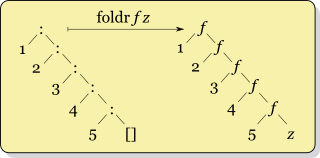
\includegraphics[width=0.4\textwidth]{pictures/Right-fold-transformation.png}
		}%
		\subfigure[Falten von links]{%
			\label{fig:LeftFold}
			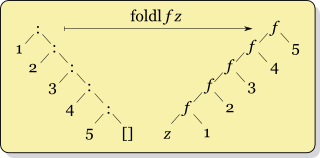
\includegraphics[width=0.4\textwidth,scale=0.5]{pictures/Left-fold-transformation.png}
		}%		
	\end{center}
	\caption{%
		Veranschaulichung des Faltens anhand von Listen \cite{HaskellWikiFold18}
	}%
	\label{fig:RightLeftFold}
\end{figure}

Das Faltbeispiel der Summen- und Produktfunktion aus Listing \ref{FoldSumPS} ist semantisch kompatibel mit Abbildung \ref{fig:RightLeftFold}, auch wenn Arrays statt Listen angewendet werden. Sowohl die Summe als auch das Produkt werden über \emph{foldl} ausgedrückt. Als Funktion und Akkumulator dient bei der Summe die binäre Funktion \lstinline[language=purescript, columns=fixed]{+} und \lstinline[language=purescript, columns=fixed]{0} als neutrales Element, bei dem Produkt \lstinline[language=purescript, columns=fixed]{*} und \lstinline[language=purescript, columns=fixed]{1}. 
\newpage
\begin{lstlisting}[language=purescript, style=numbered-and-boxed, caption=Falten in PureScript, label=FoldSumPS]
module Main where

import Prelude
import Data.Foldable

sum :: forall a f. Foldable f => Semiring a => f a -> a
sum = foldl (+) zero

product :: forall a f. Foldable f => Semiring a => f a -> a
product = foldl (*) one

resSum = sum [1, 2, 3]
resPro = product [1, 2, 3]
\end{lstlisting}

Listing \ref{FoldSumJS} zeigt am Beispiel des Faltens, wie Funktionen höherer Ordnung nach JavaScript übersetzt werden können. Da es sich bei \emph{Foldable} um eine Typklasse handelt, ist das Übersetzungsmuster gemäß des in Abschnitt \glqq \ref{lbl:Typeclasses} \nameref{lbl:Typeclasses}\grqq{} beschriebenen.

\begin{lstlisting}[language=javascript, style=numbered-and-boxed, caption=Falten in JavaScript, label=FoldSumJS]
var Prelude = require("../Prelude");
var Data_Foldable = require("../Data.Foldable");
var Data_Semiring = require("../Data.Semiring");

var sum = function (dictFoldable) {
	return function (dictSemiring) {
		return Data_Foldable.foldl(dictFoldable)(Data_Semiring.add(dictSemiring))(Data_Semiring.zero(dictSemiring));
	};
};

var product = function (dictFoldable) {
	return function (dictSemiring) {
		return Data_Foldable.foldl(dictFoldable)(Data_Semiring.mul(dictSemiring))(Data_Semiring.one(dictSemiring));
	};
};

var resSum = sum(Data_Foldable.foldableArray)(Data_Semiring.semiringInt)([ 1, 2, 3 ]);
var resPro = product(Data_Foldable.foldableArray)(Data_Semiring.semiringInt)([ 1, 2, 3 ]);
\end{lstlisting}

Es wird also analog die Typklasse \emph{Foldable} aus PureScript als Object Type (Klasse) in JavaScript repräsentiert. Die Typinstanz für die Datenstruktur Array ist ein Objekt (Type Class Dictionary) mit der Bezeichnung \emph{foldableArray}, welches ähnlich wie in Abschnitt \ref{lbl:Typeclasses} Listing \ref{Data.SemiringJS} beim Objekt \emph{semiringInt} die Implementierung des Faltens als Foreign Function Import zugewiesen bekommt. Dieses Type Class Dictionary wird als Argument übergeben, zzgl. einer Berechnungsfunktion und der Datenstruktur (Listing \ref{FoldSumJS}, je Zeile 17 und 18). Listing \ref{FoldFFIJS} zeigt, wie das Falten in JavaScript implementiert ist.

\begin{lstlisting}[language=javascript, style=numbered-and-boxed, caption=Falten als Native-Implementierung in JavaScript, label=FoldFFIJS]
exports.foldrArray = function (f) {
	return function (init) {
		return function (xs) {
			var acc = init;
			var len = xs.length;
			for (var i = len - 1; i >= 0; i--) {
				acc = f(xs[i])(acc);
			}
			return acc;
		};
	};
};

exports.foldlArray = function (f) {
	return function (init) {
		return function (xs) {
			var acc = init;
			var len = xs.length;
			for (var i = 0; i < len; i++) {
				acc = f(acc)(xs[i]);
			}
			return acc;
		};
	};
};
\end{lstlisting}

Es wird deutlich, dass das Falten nicht mit Rekursion, sondern Schleifen umgesetzt ist. Den Unterschied zwischen von links und rechts Falten, erkennt man an den jeweiligen Schleifenköpfen. Das Array \emph{xs} wird einmal von rechts und einmal von links durchlaufen. Der Parameter \emph{init} hält den Initialwert des Akkumulators, dessen Variable \emph{acc} heißt.

Die Übergabe und Rückgabe von Funktionen in Funktionen höherer Ordnung gestaltet sich als intuitiv, denn in JavaScript sind Funktionen ebenfalls First-Class-Citizens. Die Berechnungsfunktion namens \emph{f} wird einfach als Argument übergeben und in den Zeilen 7 und 20 jeweils mit dem aktuellen Array-Element und Akkumulatorwert aufgerufen.


\chapter{Funktoren, Applicatives, Monaden}
In der Prelude werden drei Typklassen definiert, die wesentlich für die Handhabung von Seiteneffekten in PureScript sind -  \emph{Functor}, \emph{Applicative} und \emph{Monad} \cite[][S. 68]{Freeman17}. 

\begin{wrapfigure}{r}{0.5\textwidth} % Inline image example
	\begin{center}
		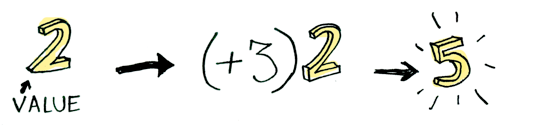
\includegraphics[width=0.45\textwidth]{Pictures/value-apply.png}
	\end{center}
	\caption{Wert und einfache Funktionsanwendung mit ihm \cite[][]{AdityaBhargava13}}
	\label{fig:SimpleValue}
\end{wrapfigure}

Rein funktionale Programmiersprachen kennen keine Seiteneffekte - zumindest keine Unkontrollierten. Das bedeutet Funktionen können \glqq nicht einfach so\grqq{} einen Zustand, wie den Inhalt einer Variable, ändern. Sie liefern bei gleichen Parametern, bei jedem Aufruf, immer das gleiche Resultat (siehe Abbildung \ref{fig:SimpleValue}). Ein wesentlicher Vorteil von dieser selbst auferlegten Beschränkung ist, dass es viel leichter als in imperativen Sprachen ist, Beweisführungen, oder zumindest Schlussfolgerungen, über die Korrektheit von Funktionen anzustellen. Dies fängt bereits bei den Vorzügen von unveränderlichen gegenüber veränderlichen Datenstrukturen an - gerade bei Nebenläufigkeit. Wenn Funktionen allerdings keine Zustände ändern können, gelangt man spätestens bei IO-Operationen an den Punkt, dass irgendwie mit der Welt außerhalb des eigenen Programms interagiert werden muss. Dies geht auch in rein funktionalen Sprachen nur über Seiteneffekte - allerdings Seiteneffekte, die nur in eigenen Berechnungskontexten, abgeschottet vom Rest unseres Programms, auftreten dürfen \cite[Kap. Input and Output]{Haskell11}.

Genau an dieser Stelle halten Konzepte wie Monaden aus der Mathematik (Kategorientheorie) in der Informatik Einzug. Der Weg zum Verständnis von Monaden führt über Funktoren und Applicatives, da aufgrund der Typklassenhierarchie eine Monade auch immer ein Applicative und ein Applicative ein Funktor ist. 

\section{Funktoren}
\begin{wrapfigure}[6]{r}{.52\textwidth}
	\begin{lstlisting}[aboveskip=-1em, language=purescript, caption=Typklasse Functor, label=FunctorTCPS]
	class Functor f where
		map :: forall a b. (a -> b) -> f a -> f b
	\end{lstlisting}
\end{wrapfigure}

Die Typklasse Funktor definiert eine Klasse für alle Typkonstruktoren \emph{f}, die eine map-Operation unterstützen - siehe Listing \ref{FunctorTCPS}. Die parametrisierten Typen Array oder Maybe sind bspw. Funktoren, da sie eine Instanz zur Typklasse Funktor definieren (dazu später mehr) \cite[][S. 29, 33]{Freeman17}. Die Map-Funktion nimmt als erstes Argument eine Funktion von einem Typ \emph{a} in einen Typ \emph{b} an, als zweites einen Typ \emph{f} von \emph{a} und gibt einen Typ \emph{f} von \emph{b} zurück, indem sie die Funktion von \emph{a} nach \emph{b} auf den Typ \emph{f} von \emph{a} anwendet. Damit handelt es sich bei \emph{map} um eine Funktion höherer Ordnung. 

Funktoren werden sich gerade in diesem Szenario oftmals als Container vorgestellt. Eine präzisere Vorstellung wäre es sich einen Funktor als Berechnungskontext vorzustellen, in dem Seiteneffekte auftreten dürfen \cite[Kap. Functors, Applicative Functors and Monoids, Abschn. Functors redux]{Haskell11}. Denn über den konkreten Berechnungskontext (Wertkonstruktor eines Funktors) entscheidet sich, was das Resultat einer Funktionsanwendung sein wird \cite{AdityaBhargava13}.

Bevor wir uns im Anschluss einem konkreten Beispiel mit Funktoren in PureScript und dessen Übersetzung nach JavaScript widmen, soll im nächsten Unterabschnitt das beschriebene Konzept zunächst visualisiert werden.

\subsection{Funktoren in Bildern am Beispiel von Maybe}
Bei der Visualisierung des Funktorkonzepts wird sich des Algebraischen Datentyps \emph{Maybe} als Beispiel bedient. Listing \ref{MaybeFunktorPS} wiederholt noch einmal die Definition von \emph{Maybe} mit dessen Wertkonstruktoren \emph{Nothing} und \emph{Just}.

 \begin{wrapfigure}[9]{r}{.52\textwidth}
	\begin{lstlisting}[aboveskip=-1em, language=purescript, caption=ADT Maybe u. Funktorinstanz, label=MaybeFunktorPS]
	data Maybe a = Nothing | Just a
	
	instance functorMaybe :: Functor Maybe where
		map fn (Just x) = Just (fn x)
		map _  _        = Nothing
	\end{lstlisting}
\end{wrapfigure}

Um eine Funktion auf den Wert in einem Funktor anwenden zu können, ohne den Wert vorher auszupacken, bedarf es einer weiteren Funktion, in der definiert ist, wie die Funktionsanwendung durchgeführt werden soll - und das macht \emph{map}. 

\begin{wrapfigure}{r}{0.5\textwidth} % Inline image example
	\begin{center}
		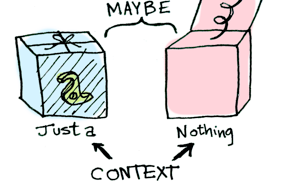
\includegraphics[width=0.4\textwidth]{Pictures/context.png}
	\end{center}
	\caption{Maybe Context \cite[][]{AdityaBhargava13}}
	\label{fig:ContextMaybe}
\end{wrapfigure}

Anhand der Wertkonstruktoren, des Berechnungskontextes, wird entschieden, welche Auswirkungen die Anwendung einer Funktion hat. Abbildung \ref{fig:ContextMaybe} veranschaulicht dies. Je nachdem, ob ein \emph{Just} von etwas oder ein \emph{Nothing} vorliegt, muss die Anwendung einer Funktion, nennen wir sie \emph{fn}, unterschiedliche Auswirkungen haben (Seiteneffekt). In Listing \ref{MaybeFunktorPS} ist die Funktorinstanz von Maybe zur Typklasse Funktor aus Listing \ref{FunctorTCPS} aufgeführt.

Im Folgenden besprechen wir beide Definitionen von Map, je nachdem welches Pattern greift. Es beginnt mit dem Fall, dass Map eine Funktion \emph{fn} bekommt und ein \emph{Just} mit einem Wert \emph{x} eines Typen \emph{a}. Gehen wir zum besseren Verständnis davon aus, der Typ wäre in einem konkreten Fall \emph{Int} und wir würden eine Funktion auf einen im Berechnungskontext gebundenen Wert \emph{2} anwenden wollen, die diesen mit einem freien Wert \emph{3} addiert (siehe Abbildung \ref{fig:MaybeJust}).

\begin{figure}[htb!]
	\centering
	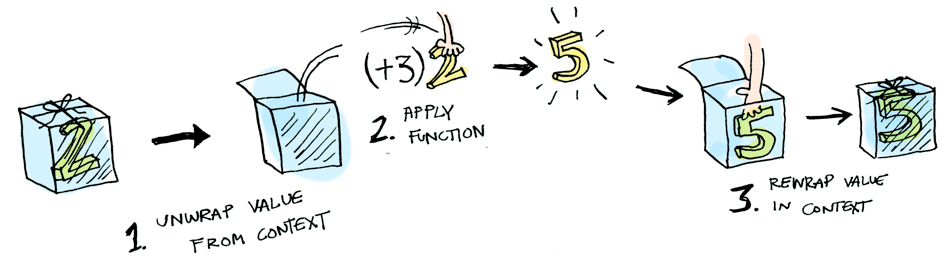
\includegraphics[width=0.75\textwidth]{Pictures/fmap-just.png}
	\caption{Funktionsanwendung auf ein Just von 2 \cite[][]{AdityaBhargava13}}
	\label{fig:MaybeJust}
\end{figure}

In dem Fall ist \emph{map} so definiert, dass intern die Funktion auf den Wert \emph{x = 2} angewendet wird. Anschließend wird das Ergebnis, hier \emph{x = 5}, über den Wertkonstruktor \emph{Just} in einem neuen Berechnungskontext (Funktor) gekapselt und dieser zurückgegeben.

Wenn der andere Fall eintritt, dass \emph{map} eine Funktion bekommt und ein \emph{Nothing}, muss \emph{map} abweichend definiert sein. Denn auf was sollte die Funktion angewendet werden, wenn \emph{Nothing} ja gar keinen Wert intern bereithält.

\begin{figure}[htb!]
	\centering
	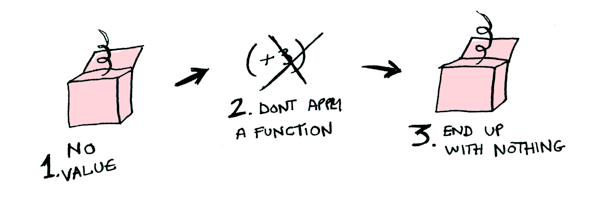
\includegraphics[width=0.55\textwidth]{Pictures/fmap-nothing.png}
	\caption{Funktionsanwendung auf Nothing \cite[][]{AdityaBhargava13}}
	\label{fig:MaybeNothing}
\end{figure}

Wie in der Definition von \emph{map} in Listing \ref{MaybeFunktorPS} zu sehen und durch Abbildung \ref{fig:MaybeNothing} visualisiert, ist das vorgeschriebene Verhalten also, dass ohne Funktionsanwendung wieder ein \emph{Nothing} zurückgegeben wird.

Typinstanzen der Typklasse \emph{Functor} müssen darüber hinaus zwei Gesetzmäßigkeiten bei der Definition ihrer \emph{map}-Funktion einhalten:

\begin{itemize}
	\item Identity Law: \lstinline[language=purescript, columns=fixed]{map identity xs = xs}
	\item Composition Law: \lstinline[language=purescript, columns=fixed]{map g (map f xs) = map (g <<< f ) xs}
\end{itemize}

Diese Gesetze garantieren, dass nicht der Berechnungskontext (Funktor) verändert wird, sondern nur der Wert. Das Gesetz der Identität sagt aus, dass wenn die Identitätsfunktion auf einen Funktor \emph{xs} angewendet wird, der originale Funktor zurückgegeben werden muss. Das macht Sinn, da die Identitätsfunktion ihre Eingabe nicht modifiziert. Das Gesetz der Komposition sagt aus, dass die Funktionsanwendung einer Funktion \emph{f} auf einen Funktor \emph{xs} über \emph{map} und die anschließende Funktionsanwendung einer weiteren Funktion \emph{g} auf dieselbe Weise über den resultierenden Funktor, das gleiche Resultat erzeugen muss, wie wenn man die Komposition der beiden Funktion \emph{g} und \emph{f} direkt auf den Funktor über \emph{map} angewendet hätte \cite[][S. 69]{AdityaBhargava13}. Der Infix-Operator \lstinline[language=purescript, columns=fixed]{<<<} beschreibt die Backwards-Komposition zweier Funktionen (\emph{g} nach \emph{f}) \cite[][S. 28]{Freeman17}.

\subsection{Funktoren in PureScript}
Dieser Unterabschnitt soll die Nutzung von Funktoren in PureScript an Beispielen verdeutlichen. Die Übersetzung nach JavaScript der hier aufgeführten Beispiele wird im nächsten Unterabschnitt aufgezeigt und besprochen.

Zunächst greifen wir  in Listing \ref{FunctorExamplePS} die, durch Bilder illustrierten, Beispiele mit dem Funktor \emph{Maybe} des letzten Unterabschnitts auf. Die unäre Funktion wird jeweils auf ein \emph{Just} von 2 und auf ein \emph{Nothing} angewendet. Durch das in der Definition von \emph{map} verwendete Pattern Matching wird der Wert 2 aus dem Funktor geholt, die Funktion mit ihm als Argument aufgerufen und das Ergebnis dessen in einen neuen Funktor gesteckt. Bei \emph{Nothing} wird ohne Funktionsanwendung \emph{Nothing} zurückgegeben.

\begin{lstlisting}[language=purescript, style=numbered-and-boxed, caption=Beispiel mit Funktoren in PS, label=FunctorExamplePS]
module Main where

import Prelude
import Data.Maybe

x = map (\x -> x + 3) (Just 2) -- x = (Just 5)
y = map (\x -> x + 3) Nothing  -- y = Nothing
\end{lstlisting}

Arrays und auch Funktionen sind ebenfalls Funktoren. In Listing \ref{FunctorExample2PS} wird zunächst eine unäre Funktion auf ein Array von Ganzzahlen angewendet. Wenn \emph{map} als Wert und Funktor eine Funktion bekommt, wirkt sich dies wie eine Funktionskomposition aus.

\begin{lstlisting}[language=purescript, style=numbered-and-boxed, caption=Weitere Funktoren in PS, label=FunctorExample2PS]
module Main where

import Prelude
import Data.Array

a = map (\x -> x + 1) [1, 2, 3, 4, 5] -- a = [2,3,4,5,6]
b = map (\x -> x + 3) (\x -> x + 2)   -- (b 1) = 6
\end{lstlisting}

Schauen wir uns zur Verdeutlichung der genauen Mechanik einmal die Implementierung der Typklasse Funktor im Falle der Instanzen für Arrays und Funktionen an. In Listing \ref{FunctorArrayFunctionPS} sind die Typinstanzen und die Implementierung der Funktion \emph{compose} angegeben. Diese wird in der Realität über mehrere Ebenen der Typklassenhierarchie geschliffen. Das soll an dieser Stelle aber nicht Gegenstand der Betrachtung sein. Die Implementierung der \emph{map}-Funktion für Arrays wird über einen Foreign Function Import aus JavaScript bereitgestellt (Listing \ref{FunctorArrayImplJS}).

\noindent\begin{minipage}[t]{.48\textwidth} 
	\hspace*{0pt}\begin{lstlisting}[language=purescript, style=only-rect, caption= Typinstanzen für Arrays und Funktionen PS, label=FunctorArrayFunctionPS]
instance functorArray :: Functor 
	Array where
	map = arrayMap

instance functorFn :: Functor
	((->) r) where
	map = compose

-- imported over several modules
compose f g x = f (g x)	
	\end{lstlisting}
\end{minipage}% 
% 
\hfill% 
\begin{minipage}[t]{.50\textwidth} 
	\hspace*{0pt}\begin{lstlisting}[language=javascript, style=only-rect, caption= Native JavaScript Impl., label=FunctorArrayImplJS] 
exports.arrayMap = function (f) {
	return function (arr) {
		var l = arr.length;
		var result = new Array(l);
		for (var i = 0; i < l; i++) {
			result[i] = f(arr[i]);
		}
		return result;
	};
};
	\end{lstlisting}
\end{minipage}
\hfill% 

Bezüglich der Mechanik bei Arrays lässt sich nun sagen, dass ein neues Array (Funktor) \emph{result} erzeugt wird, die Funktion \emph{f} auf jedes Element des alten Arrays (Funktors) \emph{arr} angewendet wird und das Resultat dieser Funktionsanwendung jeweils im neuen Funktor \emph{result} abgelegt wird. 

Die Mechanik bei Funktionen ist, wie es vom Verhalten der \emph{map}-Anwendung bereits zu vermuten war, die der Komposition von Funktionen, wie sie auch in anderen Sachverhalten eingesetzt wird. Es wird eine Funktion \emph{f} entgegen genommen, eine weitere Funktion \emph{g} als Funktor und eine neue Funktion (Funktor) zurückgegeben, in der zunächst \emph{g} auf den Wert \emph{x} angewendet wird und anschließend \emph{f} auf das Ergebnis davon. Das heißt in unserem konkreten Fall wird die Addition mit dem Wert 2 vor der Addition mit dem Wert 3 durchgeführt.

\subsection{Übersetzung nach JavaScript}
Im Folgenden wird die Übersetzung der Codebeispiele mit Funktoren des vorangegangenen Unterabschnitts dargestellt und erläutert. In Listing \ref{FunctorExampleJS} ist die Übersetzung von dem Maybe-Listing \ref{FunctorExamplePS} aufgeführt, in Listing \ref{FunctorExample2JS} die des Array- und Funktionen-Listings \ref{FunctorExample2PS}.

Da es sich bei \emph{Functor} um eine Typklasse handelt, ist das Übersetzungsmuster gemäß des in Abschnitt \glqq \ref{lbl:Typeclasses} \nameref{lbl:Typeclasses}\grqq{} beschriebenen. Es wird also analog die Typklasse \emph{Functor} aus PureScript als Object Type (Klasse) in JavaScript repräsentiert. Die Typinstanz für den ADT \emph{Maybe} ist ein Objekt (Type Class Dictionary) mit der Bezeichnung \emph{functorMaybe}, welches die Implementierung der \emph{map}-Funktion für \emph{Maybe} definiert.  In dieser wird auf die Übersetzung der Wertkonstruktoren \emph{Just a} und \emph{Nothing} des ADT \emph{Maybe} zurückgegriffen. Deren Übersetzung gestaltet sich analog zur Übersetzung der Werkkonstruktoren des Listen-ADT's aus Listing \ref{ADTJS} aus Abschnitt \glqq \ref{sec:ADT} \nameref{sec:ADT}\grqq{}. Zum besseren Verständnis der Mechanik seien die zuvor genannten Entitäten dennoch in Listing \ref{ADTMaybeFunctorJS} aufgeführt. Auf weiterführende Beschreibungen wird allerdings verzichtet. Zur Reduzierung der Länge des Listings sind an geeigneten Stellen Zeilenumbrüche entfernt worden.

\begin{lstlisting}[language=javascript, style=numbered-and-boxed, caption=Übersetzung der Typklasse \emph{Functor} und Typinstanz \emph{functorMaybe}, label=ADTMaybeFunctorJS]
// ../Data.Functor/index.js
var Functor = function (map) { this.map = map; };

var map = function (dict) { return dict.map; };

// ../Data.Maybe/index.js
var functorMaybe = new Data_Functor.Functor(function (v) {
	return function (v1) { // v1 ist ein Objekt, v eine Funktion
		if (v1 instanceof Just) { return new Just(v(v1.value0)); };
		return Nothing.value;
	};
});

var Nothing = (function () { // kann oben als v1 auftreten 
	function Nothing() { };
	Nothing.value = new Nothing(); 
	return Nothing; 
})();

var Just = (function () { // kann oben als v1 auftreten 
	function Just(value0) { this.value0 = value0; };
	Just.create = function (value0) { return new Just(value0); };
	return Just; 
})();
\end{lstlisting}

Richten wir unser Augenmerk nun auf Listing \ref{FunctorExampleJS}. Es wird in Zeile 4 ein neues \emph{functorMaybe} Type Class Dictionary (Objekt in JavaScript, Typinstanz in PureScript) erzeugt. Dieses bekommt\footnote{aufgrund des Currying's wird auch in diesen und weiteren Beispielen partielle Anwendung in JavaScript genutzt, weshalb manche Formulierung unpräzise ist, aber es steht gerade anderes im Vordergrund} in diesem Fall eine unäre Additionsfunktion (oben \emph{v} genannt) und ein Objekt \emph{Just} (oben \emph{v1}) mit dem Wert 2 (oben \emph{v1.value0}). Das Type Class Dictionary \emph{functorMaybe} wird der freien Funktion \emph{map} des Moduls \emph{Data.Functor} als Argument übergeben. Diese Funktion ruft anschließend die Klassenfunktion \emph{map} auf, deren Implementierung die übergebene Additionsfunktion und das Funktorobjekt entsprechend des bereits zuvor beschriebenen Mechanismuses des Maybe-Funktors verwertet (Zeile 9, Listing \ref{ADTMaybeFunctorJS}). Der Fall mit dem Wertkonstruktor \emph{Nothing} in Zeile 10 bis 12 aus Listing \ref{FunctorExampleJS} ist im Aufrufverhalten gleich, wird aber unterschiedlich verwertet (Zeile 10, Listing \ref{ADTMaybeFunctorJS}).

\begin{lstlisting}[language=javascript, style=numbered-and-boxed, caption=Übersetzung des Maybe-Funktorenbeispiels nach JS, label=FunctorExampleJS]
var Data_Functor = require("../Data.Functor");
var Data_Maybe = require("../Data.Maybe");
var Data_Semiring = require("../Data.Semiring");
var Prelude = require("../Prelude");

var x = Data_Functor.map(Data_Maybe.functorMaybe)(function (x1) {
	return x1 + 3 | 0;
})(new Data_Maybe.Just(2));

var y = Data_Functor.map(Data_Maybe.functorMaybe)(function (x1) {
	return x1 + 3 | 0;
})(Data_Maybe.Nothing.value);
\end{lstlisting}

 \begin{wrapfigure}[10]{r}{.52\textwidth}
	\begin{lstlisting}[aboveskip=-1em, language=javascript, caption=Auszug Funktor Array u. Function, label=ArrayFunctionFunctorJS]
var functorArray = new Functor($foreign.arrayMap);

var compose = function (f) {
	return function (g) {
		return function (x) {
			return f(g(x)); }; }; });	
	\end{lstlisting}
\end{wrapfigure}

Kommen wir nun zur Übersetzung von Arrays und Funktionen als Funktoren in Listing \ref{FunctorExample2JS}. Da Arrays ein in die Sprache PureScript direkt eingebauter Datentyp sind, ist das Aufrufverhalten einfacher als bei \emph{Maybe}. Das Type Class Dictionary \emph{functorArray} bekommt ohne Umschweife bei Erzeugung aus der Funktorklasse die Implementierung von \emph{arrayMap} (Listing \ref{FunctorArrayImplJS}) übergeben. Da die exakte Umsetzung des Funktors \emph{functorFn}, wie bereits zuvor erwähnt, weitere Typklassen einführen würde, sei auch an dieser Stelle in Listing \ref{ArrayFunctionFunctorJS} nur die Implementierung in JavaScript der \emph{compose}-Funktion angeben. Das Aufrufverhalten gestaltet sich jedoch wieder analog zu dem von \emph{Maybe}.

\begin{lstlisting}[language=javascript, style=numbered-and-boxed, caption=Übersetzung des Beispiels mit Array und Funktion als Funktor nach JS, label=FunctorExample2JS]
var a = Data_Functor.map(Data_Functor.functorArray)(function (x) {
	return x + 1 | 0;
})([ 1, 2, 3, 4, 5 ]);

var b = Data_Functor.map(Data_Functor.functorFn)(function (x) {
	return x + 3 | 0;
})(function (x) {
	return x + 2 | 0;
});
\end{lstlisting}

\section{Applicatives}
Applicatives sind eine Subklasse von Funktoren und erweitern diese um zwei weitere Funktionen.
\begin{itemize}
	\item apply - wie map, nur, dass auch die Funktion, die angewendet werden soll, bereits in einem Funktor steckt \cite[][S. 84]{Freeman17}
	\item pure - um Werte in einen Funktor zu betten, in einen Berechnungskontext zu heben \cite[][S. 86]{Freeman17}
\end{itemize}
In PureScript steht die Typklasse \emph{Applicative} nicht direkt unter \emph{Functor} in der Hierarchie, sondern \emph{Functor} wird zunächst durch eine Typklasse names \emph{Apply} erweitert und diese anschließend von \emph{Applicative}. In Listing \ref{ApplicativeTCPS} wird dies dargestellt und auf welcher Hierarchieebene welche der beiden Funktionen wie definiert ist.

\begin{lstlisting}[language=purescript, style=numbered-and-boxed, caption=Typklasse Applicative, label=ApplicativeTCPS]
class Functor f where
	map :: forall a b. (a -> b) -> f a -> f b

class Functor f <= Apply f where
	apply :: forall a b. f (a -> b) -> f a -> f b

class Apply f <= Applicative f where
	pure :: forall a. a -> f a
\end{lstlisting}

Bevor wir uns im Anschluss einem konkreten Beispiel mit Applicatives in PureScript und dessen Übersetzung nach JavaScript widmen, soll im nächsten Unterabschnitt das beschriebene Konzept zunächst visualisiert werden.

\subsection{Applicatives in Bildern am Beispiel von Maybe}
Bei der Visualisierung des Konzepts von Applicatives wird sich, wie zuvor bei Funktoren, des Algebraischen Datentyps \emph{Maybe} als Beispiel bedient. In Listing \ref{MaybeApplicativePS} ist die Typinstanz für \emph{Maybe} als Funktor nochmals wiederholt und die neuen Typinstanzen für die Typklassen \emph{Apply} und \emph{Applicative} aufgeführt.

\begin{lstlisting}[language=purescript, style=numbered-and-boxed, caption=Applicative-Intanz Maybe, label=MaybeApplicativePS]
instance functorMaybe :: Functor Maybe where
	map fn (Just x) = Just (fn x)
	map _  _        = Nothing

instance applyMaybe :: Apply Maybe where
	apply (Just fn) x = fn <$> x
	apply Nothing   _ = Nothing
	
instance applicativeMaybe :: Applicative Maybe where
	pure = Just
\end{lstlisting}

An der Definition der Typinstanz \emph{applyMaybe} ist zu sehen, dass die Funktion \emph{apply} ihr erstes Argument in einem Funktor haben möchte. Das ist der Unterschied zur Funktion \emph{map} bei Funktoren. Durch Abbildung \ref{fig:MaybeApplicativeJust} wird das Vorgehen visualisiert dargestellt. Für den Fall, dass das erste Argument eine Funktion in einem \emph{Just} ist und das zweite Argument ein Wert in einem Funktor, werden beide durch das Pattern Matching ausgepackt. Anschließend wird die Funktion durch \emph{map}, vertreten durch seinen Infix-Alias \emph{<\$>}, auf den Wert angewendet und das Resultat wieder in einen Funktor eingebettet \cite[][S. 84]{Freeman17}.

\begin{figure}[htb!]
	\centering
	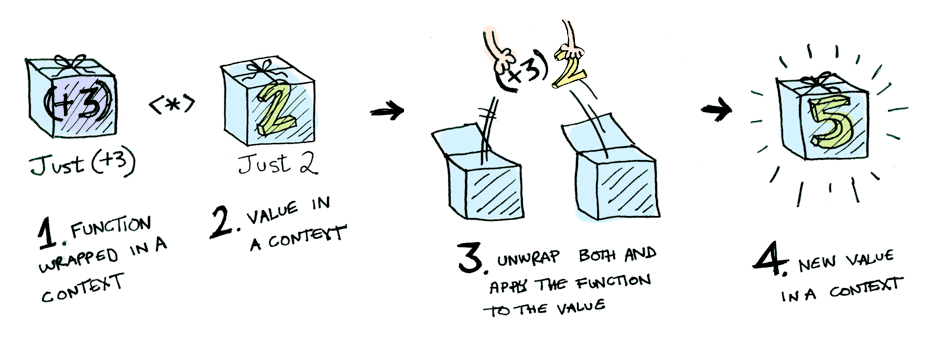
\includegraphics[width=0.75\textwidth]{Pictures/applicative-just.png}
	\caption{Funktionsanwendung aus einem Just auf ein Just von 2 \cite[][]{AdityaBhargava13}}
	\label{fig:MaybeApplicativeJust}
\end{figure}

Für den Fall, dass das erste Argument ein \emph{Nothing} ist, wird, wie bei Funktoren auch, wieder ein \emph{Nothing} zurückgeliefert. Bei Funktoren gab es keinen Wert, auf den die Funktion \emph{fn} hätte angewendet werden können. Jetzt gibt es keine Funktion \emph{fn}, da das erste Argument ein \emph{Nothing} ist und den Wert ohne Funktionsanwendung einfach wieder zurückzugeben, würde zu einem Typfehler führen. Denn das zweite Argument ist vom Typ \emph{a} bevor es durch eine Funktion von \emph{a} nach \emph{b} zu einem Typ von \emph{b} wird. Ohne diese Funktion zu haben, bleibt uns keine andere Option als Nothing zu erzeugen.

In der Typinstanz \emph{applicativeMaybe} wird die konstante Funktion \emph{pure} für \emph{Maybe} definiert, indem sie den Wertkonstruktor \emph{Just} zugewiesen bekommt.

Die Typinstanzen der Typklasse \emph{Applicative} bzw. \emph{Apply} müssen bei der Implementierung der Funktionsdeklarationen ebenso wie Funktoren einige Gesetze einhalten. Diese sollen an dieser Stelle aber nicht im Detail besprochen werden.

\subsection{Applicatives in PureScript}
Dieser Unterabschnitt soll die Nutzung von Applicatives und vor allem ihre Vorzüge im Vergleich zu Funktoren an Beispielen verdeutlichen. Die Übersetzung nach JavaScript der hier aufgeführten Beispiele wird im nächsten Unterabschnitt besprochen.

In Listing \ref{ApplicativeExamplePS} ist der bereits erwähnte Unterschied zu Funktoren demonstriert. Dort wird neben der Funktion \emph{apply} auch deren Infix-Alias \emph{<*>} genutzt. Im Gegensatz zu \emph{map} dürfen sich die Funktionen ebenfalls bereits in einem Funktor befinden.

\begin{lstlisting}[language=purescript, style=numbered-and-boxed, caption=Beispiel mit Applicatives in PS, label=ApplicativeExamplePS]
module Main where

import Prelude
import Data.Maybe

a = apply (Just \x -> x + 3) (Just 2) 			  	 -- (Just 5)
b = [(\x -> x * 2), (\x -> x + 2)] <*> [1, 2, 3] -- [2,4,6,3,4,5]
c = [(\x y -> x * y), (\x y -> x + y)] <*> pure 2  <*> [1, 2, 3]
\end{lstlisting}

Zeile 6 zeigt, dass \emph{apply} im Grunde wie \emph{map} funktioniert, wie wir auch schon anhand ihrer Definition erkennen konnten. Das Beispiel ist im Resultat äquivalent mit dem in Listing \ref{FunctorExamplePS} bei Funktoren. Dadurch, dass die Funktion in einem Funktor sein darf, eröffnen sich aber auch Möglichkeiten, welche die Mächtigkeit von einfachen Funktoren übersteigen. Ein erstes Beispiel dafür ist in Zeile 7 zu sehen. Ein Array ist ebenso ein Funktor und kann damit, gefüllt mit Funktionen, genutzt werden. Als Auswirkung wird zunächst die erste Funktion auf die Elemente des Arrays, dass als Wert gedient hat, angewendet und im Anschluss die zweite Funktion auf dieselben Ursprungswerte. Als Ergebnis entsteht ein Array, dass die Resultate der beiden Funktionsanwendungen in sich vereint. 

In Zeile 7 wird kurz die praktische Nutzung von \emph{pure} demonstriert, was einen einfachen Wert in den Berechnungskontext hebt. Die vorherigen unären Funktionen sind jetzt binär, damit der Wert 2 und jeweils ein Element des Arrays wie zuvor in Zeile 6 miteinander verrechnet werden können. Es entsteht demnach das gleiche Array als Ergebnis.

Es deutete sich bereits an, dass die praktische Ausnutzung des Unterschieds von Funktoren zu Applicatives etwas mit der Anzahl der Argumente einer Funktion zu tun haben könnte. Dies soll nachfolgend, durch Listing \ref{ApplicativeExample2PS} begleitet, bestätigt werden.

Wenn wir bei Funktoren eine unäre Funktion auf einen Wert in einem Berechnungskontext anwenden, erhalten wir einen Wert in einem neuen Berechnungskontext (Zeile 1). Wird allerdings mindestens eine binäre Funktion angewendet, ergibt dies durch die partielle Anwendung eine Funktion, die um ein Argument kürzer ist (Zeile 2). Dies ist kein wirklicher Unterschied zu Zeile 1, denn dort wurde durch die partielle Anwendung eine Funktion von einem Argument auf eine Funktion von keinem Argument reduziert, also auf eine konstante Funktion bzw. Wert. In beiden Fällen haben wir prinzipiell das Problem: \glqq Und wie solls jetzt \textbf{weitergehen}?\grqq{}. Entweder wir legen selbst Hand an und holen unseren Wert oder Funktion aus dem Berechnungskontext durch Pattern Matching heraus, verwerten ihn und heben ihn wieder in einen neuen Kontext hoch (Zeile 4 - 6) oder wir bedienen uns etwas Vorgefertigtem. 

\begin{lstlisting}[language=purescript, style=numbered-and-boxed, caption=Grenzen von Funktoren, label=ApplicativeExample2PS]
a = (\x -> x + 3) <$> (Just 2)   -- a = (Just 5)
b = (\x y -> x + y) <$> (Just 2) -- b = (\y -> 2 + y)

c :: Maybe (Int -> Int) -> Int -> Maybe Int -- (c b 3) = (Just 5)
c (Just f) y = Just(f y)
c Nothing y = Nothing

d = lift2 (\x y -> x + y) (Just 2) (Just 3) -- d = (Just 5)
\end{lstlisting}

In Zeile 8 wird durch die Funktion \emph{lift2} aus dem Modul \emph{Control.Apply} eine Funktion, die zwei Argumente annimmt, mit diesen Argumenten in einen Berechnungskontext gehoben, die Funktion auf diese angewendet und das Resultat in einen neuen Berechnungskontext gepackt. Schön und gut, aber was ist, wenn die Funktion drei Argumente annimmt?  In diesem Modul gibt es Lift-Funktionen für Funktionen bis zu fünf Argumenten, aber etwas umständlich ist es dennoch noch und wir sind nicht in der Lage Funktionen mit einer beliebigen Anzahl Argumente zu behandeln. 

Schauen wir uns in Listung \ref{ApplicativeExample3PS} exemplarisch an, wie die Lift-Funktionen definiert sind. Es fällt auf, dass die Definition einem strikten Schema folgen, was wir statisch unendlich so weiterführen könnten. Alternativ könnten wir uns aber auch eine Funktion \emph{lift1} definieren und diese durch mehrfache partielle Anwendung auf Funktionen einer beliebigen Anzahl Argumente anwenden - solange wie es für einen spezifischen Anwendungsfall von Nöten ist.

\begin{lstlisting}[language=purescript, style=numbered-and-boxed, caption=Auszug aus \emph{Control.Apply}, label=ApplicativeExample3PS]
lift2 :: forall a b c f. Apply f => (a -> b -> c) -> f a -> f b -> f c
lift2 f a b = f <$> a <*> b

lift3 :: forall a b c d f. Apply f => (a -> b -> c -> d) -> f a -> f b -> f c -> f d
lift3 f a b c = f <$> a <*> b <*> c
\end{lstlisting}

Die Funktion \emph{lift1} gibt es bereits und nennt sich \emph{apply}. Sie ist neben der Funktion \emph{pure}, die wenn man so will Funktionen mit keinen Argumenten in einen Berechnungskontext hochhebt, das was die Typklasse \emph{Applicative} ausmacht und alles was wir brauchen. 

Listing \ref{ApplicativeExample4PS} zeigt zur Verdeutlichung nochmal die Funktionsdeklaration von \emph{apply} und anhand der Beispiele aus Listing \ref{ApplicativeExample2PS} wie sie sich bequem deklarativ, ohne Boilerplate-Code, durch Applicatives formulieren lassen.

\begin{lstlisting}[language=purescript, style=numbered-and-boxed, caption=Aneinanderkettung von Berechnungen mit Applicatives in PS, label=ApplicativeExample4PS]
-- apply :: forall a b. f (a -> b) -> f a -> f b

a = (\x y -> x + y) <$> (Just 2) <*> (Just 3) -- a = (Just 5)
b = (\x y z -> x + y + z) <$> (Just 2) <*> (Just 3) <*> (Just 5) 
-- b = (Just 10)
\end{lstlisting}

Applicatives sind also einfachen Funktoren bei Funktionen mit mehr als einem Argument überlegen. Durch die Kombination von \emph{map} und \emph{apply} können Funktionen mit beliebiger Anzahl ungebundener Argumente auf die gleiche Anzahl von Werten, die bereits in einem Berechnungskontext gebunden sind, angewendet werden. Das Ergebnis der sukzessive partiellen Funktionsanwendung ist wie bei Funktoren ein Wert in einem neuen Berechnungskontext. So scheint es kein Zufall zu sein, dass Funktoren in dem Modul \emph{Data} definiert sind und Applicatives im Modul \emph{Control}, da sie zusätzlich doch eine generische Art und Weise vorgeben, wie herkömmliche Funktionen elegant mit eingepackten Werten umgehen können. Sie erlauben im Gegensatz zu einfachen Funktoren eine Aneinanderreihung von Berechnungsschritten unter dem Standpunkt der funktionalen Sicht auf Seiteneffekte.

\subsection{Übersetzung nach JavaScript}
In diesem Unterabschnitt  wird die Übersetzung einiger Codebeispiele mit Applicatives des vorangegangenen Unterabschnitts dargestellt und erläutert. Diese sind in Listing \ref{ApplicativeSummaryPS} nochmal zusammengefasst aufgeführt.

Da es sich bei Applicatives um eine Typklasse handelt, ist das Übersetzungsmuster gemäß des in Abschnitt \glqq \ref{lbl:Typeclasses} \nameref{lbl:Typeclasses}\grqq{} beschriebenen. Es wird also analog die Typklasse \emph{Applicative} aus PureScript als Object Type (Klasse) in JavaScript repräsentiert. Die Typinstanz für den ADT \emph{Maybe} ist ein Objekt (Type Class Dictionary) mit der Bezeichnung \emph{applicativeMaybe}.  Da in der Übersetzung auf die Wertkonstruktoren \emph{Just a} und \emph{Nothing} des ADT \emph{Maybe} und auf die von Funktoren zurückgegriffen wird, lohnt ein Blick in Listing \ref{ADTMaybeFunctorJS}. Applicatives stehen in der Typklassenhierarchie unter \emph{Apply} und \emph{Functor}. Diese Beziehung wird über die Übersetzung ebenfalls deutlich. Zur Reduzierung der Länge der nachfolgenden Listings sind an geeigneten Stellen Zeilenumbrüche entfernt worden.

In Listing \ref{TypeClassApplicativeJS} ist die Übersetzung der Typklassen \emph{Apply} und \emph{Applicative} nach JavaScript dargestellt. In \emph{Apply} wird dazu auf die Übersetzung der Typklasse \emph{Functor} zurückgegriffen und in \emph{Applicative} auf die von \emph{Apply}. An dieser Stelle wird also die Beziehung zwischen diesen Typklassen deutlich und auch, dass ein Applicative auch immer ein Funktor ist, da es über die gleichen Fähigkeiten verfügt.

\begin{lstlisting}[language=javascript, style=numbered-and-boxed, caption=Übersetzung der Typklassen \emph{Apply} und \emph{Applicative}, label=TypeClassApplicativeJS]
// ../Control.Apply/index.js
var Apply = function (Functor0, apply) {
	this.Functor0 = Functor0;
	this.apply = apply;
};
var apply = function (dict) { return dict.apply; };

// ../Control.Applicative/index.js
var Applicative = function (Apply0, pure) {
	this.Apply0 = Apply0;
	this.pure = pure;
};
var pure = function (dict) { return dict.pure; };
\end{lstlisting}

Listing \ref{ADTMaybeApplicativeJS} zeigt, analog zu Funktoren in Listing \ref{ADTMaybeFunctorJS}, die Typinstanzen für \emph{Apply} und \emph{Applicative} im Falle des ADT's \emph{Maybe}.

\begin{lstlisting}[language=javascript, style=numbered-and-boxed, caption=Übersetzung der Typinstanzen für \emph{Maybe}, label=ADTMaybeApplicativeJS]
// ../Data.Maybe/index.js
var applyMaybe = new Control_Apply.Apply(
	function () { return functorMaybe; }, function (v) {
	return function (v1) { // v1 ist ein Objekt, v eine Funktion, ..
		if (v instanceof Just) { // nun auch in einem Objekt gekapselt
			return Data_Functor.map(functorMaybe)(v.value0)(v1);
		};
		if (v instanceof Nothing) {
			return Nothing.value;
		};
		throw new Error("<pattern error message skipped by author>");
	};
});

var applicativeMaybe = new Control_Applicative.Applicative(
	function () { return applyMaybe; }, Just.create);
\end{lstlisting}

Das Vorgehen unterscheidet sich nicht wesentlich von dem, welches wir bei Funktoren vorgefunden haben. Wegen der Typklassenhierarchie wird auch hier wieder auf die Typinstanzen des übergeordneten Typs zugegriffen. Die Funktion \emph{pure} wird zu einer Erstellung von einem \emph{Just} (Zeile 16). Die Funktion \emph{apply} ist, im Falle eines \emph{Just}, über den Aufruf der Funktion \emph{map} von Funktoren definiert, indem es dieser die ausgepackte Funktion (\emph{v.value0}) und den noch eingepackten Wert (\emph{v1}) übergibt. Im Fall von \emph{Nothing} passiert das gleiche wie bei Funktoren. Da es für einen anderen Fall kein definiertes Verhalten gibt, wird in einem solchen ein Fehler geworfen.

Die Übersetzung der in Listing \ref{ApplicativeSummaryPS} zusammengefassten Codebeispiele werden im Folgenden nacheinander besprochen. Es werden nur für das Verständnis nötige Imports einmalig beim ersten Listing aufgeführt.

\begin{lstlisting}[language=purescript, style=numbered-and-boxed, caption=Applicatives in PS, label=ApplicativeSummaryPS]
a = [(\x -> x * 2), (\x -> x + 3)] <*> [1, 2, 3]
b = (\x y -> x + y) <$> (Just 2) <*> (Just 3)
c = (\x y z -> x + y + z) <$> (Just 2) <*> (Just 3) <*> (Just 5)
\end{lstlisting}

\begin{wrapfigure}[16]{r}{.55\textwidth}
 \begin{lstlisting}[aboveskip=-1em, language=javascript, caption=Auszug Control.Apply, label=ArrayFunctionApplicativeJS]
exports.arrayApply = function (fs) {
	return function (xs) {
		var l = fs.length;
		var k = xs.length;
		var result = new Array(l*k);
		var n = 0;
		for (var i = 0; i < l; i++) {
			var f = fs[i];
			for (var j = 0; j < k; j++) {
				result[n++] = f(xs[j]);
			}
		}
		return result;
	};
};
\end{lstlisting}
\end{wrapfigure}

Die Übersetzung des Beispiels unter Verwendung von Arrays ist in Listing \ref{ApplicativeExample1JS} dargestellt. Wie bereits im Abschnitt über Funktoren erwähnt, ist das Aufrufverhalten beim fest in die Sprache eingebauten Typ \emph{Array} einfacher als bei Typen wie \emph{Maybe}. Analog wie in Listing \ref{ArrayFunctionFunctorJS} bereits dargestellt, bekommt das Type Class Dictionary \emph{applyArray} bei Erzeugung aus der Applyklasse direkt die Implementierung von \emph{arrayApply}  übergeben. Diese ist in Listing \ref{ArrayFunctionApplicativeJS} aufgeführt.

Das Beispiel soll verdeutlichen wie ein einfacher Aufruf von \emph{apply} realisiert wird. In Zeile 7 wird ein neues  \emph{applyArray} Type Class Dictionary (Objekt) erzeugt. Dieses hält die beiden, zuvor in einem Array abgelegten, Funktionen. Darüber hinaus bekommt es das Array von drei Werten übergeben. Das Type Class Dictionary wird der freien Funktion \emph{apply} des Moduls \emph{Control.Apply} als Argument überreicht. Diese Funktion ruft anschließend die Klassenfunktion \emph{apply} auf, was zum Aufruf von \emph{arrayApply} aus Listing \ref{ArrayFunctionApplicativeJS} führt.

\begin{lstlisting}[language=javascript, style=numbered-and-boxed, caption=Übersetzung von Applicatives mit Arrays nach JS, label=ApplicativeExample1JS]
var Control_Apply = require("../Control.Apply");
var Data_Functor = require("../Data.Functor");
var Data_Maybe = require("../Data.Maybe");

var a = Control_Apply.apply(Control_Apply.applyArray)
([ function (x) {
	return x * 2 | 0;
}, function (x) {
	return x + 3 | 0;
} ])([ 1, 2, 3 ]);
\end{lstlisting}

In der Funktion \emph{arrayApply} wird das Array von Funktionen \emph{fs} und das Array von Werten \emph{xs} angenommen. In einer ersten Schleife wird sich die jeweilige Funktion herausgenommen. In einer zweiten geschachtelten Schleife wird diese Funktion auf alle Argumente angewendet und die Resultate in einem neuen Array gespeichert. Darauf folgt die Anwendung aller weiteren Funktionen auf dieselbe Weise.

Im nachfolgenden Listing \ref{ApplicativeExample2JS} soll verdeutlicht werden, wie ein Aufruf von \emph{map} in Verbindung mit einem Aufruf von \emph{apply} übersetzt wird.

\begin{lstlisting}[language=javascript, style=numbered-and-boxed, caption=Übersetzung von Applicatives mit Maybe nach JS, label=ApplicativeExample2JS]
var b = Control_Apply.apply(Data_Maybe.applyMaybe)
(Data_Functor.map(Data_Maybe.functorMaybe)
(function (x) {
	return function (y) {
		return x + y | 0;
	};
})(new Data_Maybe.Just(2)))(new Data_Maybe.Just(3));
\end{lstlisting}

Die \emph{map}-Funktion bekommt das \emph{Just} von 2 und dieses wird an den Parameter \emph{x} gebunden. Im Anschluss bekommt die \emph{apply}-Funktion die in einem \emph{Just} gekapselte partiell aufgerufene Funktion des \emph{map}-Aufrufs sowie das \emph{Just} von 3 und ersetzt den Parameter \emph{y} mit diesem.

Bei weiteren \emph{apply}-Aufrufen wird, wie in Listing \ref{ApplicativeExample3JS} zu sehen, ein weiteres \emph{applyMaybe} Objekt nach dem gleichen Schema in den Aufruf integriert.

\begin{lstlisting}[language=javascript, style=numbered-and-boxed, caption=Übersetzung von Applicatives mit Maybe nach JS, label=ApplicativeExample3JS]
var c = Control_Apply.apply(Data_Maybe.applyMaybe)
(Control_Apply.apply(Data_Maybe.applyMaybe)
(Data_Functor.map(Data_Maybe.functorMaybe)
(function (x) {
	return function (y) {
		return function (z) {
			return (x + y | 0) + z | 0;
		};
	};
})(new Data_Maybe.Just(2)))(new Data_Maybe.Just(3)))(new Data_Maybe.Just(5));
\end{lstlisting}

\section{Monaden}
Monaden sind eine Subklasse von Applicatives und erweitern diese um eine Funktion \emph{bind}. Kurz zur Wiederholung und zur Intention von \emph{bind}:
\begin{itemize}
	\item Funktoren erlauben es durch \emph{map}, eine Funktion auf einen Wert in einem Funktor anzuwenden.
	\item Applicatives erlauben es durch \emph{apply}, eine Funktion in einem Funktor auf einen Wert in einem Funktor anzuwenden. Dadurch wird die Aneinanderreihung von Funktionsberechnungen möglich.
	\item Monaden erlauben es durch \emph{bind}, eine Funktion entgegen zu nehmen, die einen kontextlosen Wert nimmt und einen Wert in einem Kontext (Monade) zurückliefert. Die anzuwendende Funktion darf also im Gegensatz zu \emph{map} oder \emph{apply} bereits einen eingepackten Wert zurückliefern. Dadurch wird die Aneinanderreihung von Funktionsberechnungen ermöglicht, wo in jeweils jeder Funktionsberechnung entschieden werden kann, welche Berechnung auf der Basis des Ergebnisses der vorangegangen Berechnung ausgeführt werden soll. Der resultierende spezifische Berechnungskontext hängt also lediglich von der Auswertung der Funktion ab, nicht von der Definition des Pattern Matchings des Funktors (siehe bspw. Listing \ref{MaybeMonadPS}).
\end{itemize}

In PureScript gibt es auf der gleichen Hierarchieebene wo sich sich die Typklasse \emph{Applicative} befindet eine Typklasse \emph{Bind}, welche die Funktion \emph{bind} deklariert. Die Typklasse Monad erweitert eine Ebene darunter diese beiden Typklassen und bringt deren Funktionalität damit zusammen, wie in Listing \ref{MonadTCPS} zu sehen \cite[][S. 101]{Freeman17}. In der Bibliothek wird im Zusammenhang mit Monaden der Funktor in deren Funktionsdeklaration mit dem Buchstaben \emph{m} anstatt \emph{f} ausgedrückt, was aber keinen Unterschied macht.

\begin{lstlisting}[language=purescript, style=numbered-and-boxed, caption=Typklasse Monad, label=MonadTCPS]
class Functor f where
	map :: forall a b. (a -> b) -> f a -> f b

class Functor f <= Apply f where
	apply :: forall a b. f (a -> b) -> f a -> f b

class Apply f <= Applicative f where
	pure :: forall a. a -> f a

class Apply m <= Bind m where
	bind :: forall a b. m a -> (a -> m b) -> m b

class (Applicative m, Bind m) <= Monad m
\end{lstlisting}

Bevor wir uns im Anschluss einem konkreten Beispiel mit Monaden in PureScript und dessen Übersetzung nach JavaScript widmen, soll im nächsten Unterabschnitt das beschriebene Konzept zunächst visualisiert werden.

\subsection{Monaden in Bildern am Beispiel von Maybe}
Bei der Visualisierung des Konzepts von Monaden wird sich, wie zuvor bei Funktoren und Applicatives, des Algebraischen Datentyps \emph{Maybe} als Beispiel bedient. In Listing \ref{MaybeMonadPS} ist die Typinstanz für \emph{Maybe} als Funktor und Applicative nochmals wiederholt und die neuen Typinstanzen für die Typklassen \emph{Bind} und \emph{Monad} aufgeführt.

\begin{lstlisting}[language=purescript, style=numbered-and-boxed, caption=Monad-Instanz Maybe, label=MaybeMonadPS]
instance functorMaybe :: Functor Maybe where
	map fn (Just x) = Just (fn x)
	map _  _        = Nothing

instance applyMaybe :: Apply Maybe where
	apply (Just fn) x = fn <$> x
	apply Nothing   _ = Nothing

instance applicativeMaybe :: Applicative Maybe where
	pure = Just

instance bindMaybe :: Bind Maybe where
	bind (Just x) k = k x
	bind Nothing  _ = Nothing
	
instance monadMaybe :: Monad Maybe
\end{lstlisting}

An der Typinstanz \emph{bindMaybe} ist zu sehen, dass wir einen Wert in dem Monadentyp \emph{Just} oder \emph{Nothing} erwarten. Durch Abbildung \ref{fig:MaybeMonadJust} wird das Vorgehen für den ersten Fall visualisiert dargestellt. Die Funktion \emph{bind} bekommt einen Wert in einer Monade (Funktor) als erstes Argument. Durch Pattern Matching wird der Wert ausgepackt. Das zweite Argument ist eine beliebige Funktion, die einen Wert außerhalb eines Funktors erwartet und einen Wert in einem Funktor zurückliefert. Der Rückgabewert der Funktionsanwendung ist gleichzeitig der Rückgabewert von \emph{bind}.

Das bedeutet die Funktion, die als Argument angeben wird, entscheidet \textbf{wie} es \textbf{weitergeht} - was für ein Funktor genau zurückgegeben wird. Bei den Funktionen \emph{map} und \emph{apply} war das durch deren Fallunterscheidung bereits entschieden. Für den Fall von \emph{Maybe} in Listing \ref{MaybeMonadPS} ist in Zeile 13 nicht entschieden, dass wenn wir ein \emph{Just} von etwas bekommen auch wie bei \emph{map} und \emph{apply} ein \emph{Just} resultieren muss (Zeile 2 und 6). Die Funktion \emph{k} könnte auch ein \emph{Nothing} zurückliefern. In Abbildung \ref{fig:MaybeMonadJust} ist bspw. eine Funktion \emph{half} definiert, wie in Listing \ref{HalfPS} dargestellt.

\begin{lstlisting}[language=purescript, style=numbered-and-boxed, caption=Funktion mit Monad-Anwendung, label=HalfPS]
half :: Int -> Maybe Int
half x = if even x
	then Just (div x 2)
	else Nothing

retNothing = Just 20 >>= half >>= half >>= half
\end{lstlisting}

\begin{wrapfigure}[20]{r}{.55\textwidth}
	\centering
	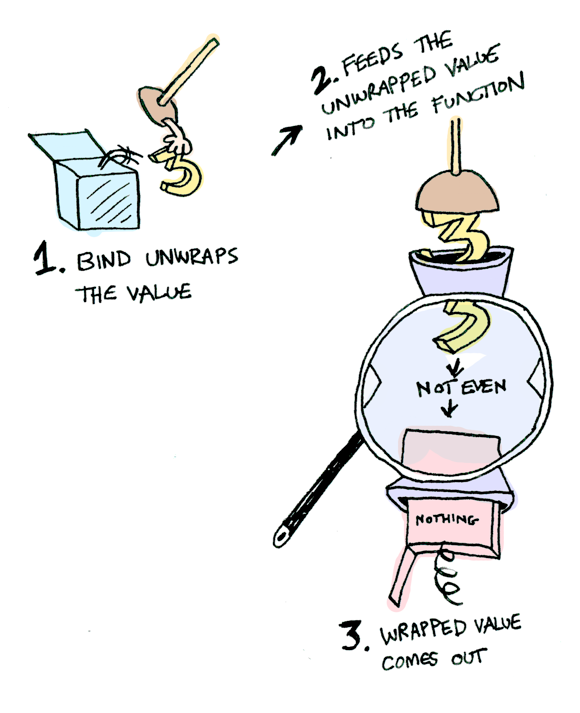
\includegraphics[width=0.4\textwidth]{Pictures/monad-just.png}
	\caption{Funktionsanwendung auf ein Just von 3, wo der Ausgang der Funktionsanwendung, die Rückgabe von \emph{bind} bestimmt \cite[][]{AdityaBhargava13}}
	\label{fig:MaybeMonadJust}
\end{wrapfigure}

Durch \emph{half} entscheidet sich, ob der Aufruf von \emph{bind} ein \emph{Just} oder ein \emph{Nothing} zurückliefern wird. Wie in Zeile 6 des Listings zu sehen, kann man dadurch eine direkte Verkettung von \emph{bind}-Aufrufen angeben. Die Funktion \emph{bind} wird dort durch deren Infix-Alias \emph{>>=} vertreten \cite[][S. 101]{Freeman17}. Aus dem ersten Aufruf resultiert ein \emph{Just 10}, wird im zweiten Aufruf von \emph{bind} ausgepackt und erneut in die Funktion \emph{half} gesteckt. Das Resultat davon ist \emph{Just 5}, was bei, dritten Aufruf von \emph{bind} in einem \emph{Nothing} endet. Alle erneuten Anwendungen würden immer in einem \emph{Nothing} enden, da die Funktion \emph{half} per Typinstanzdefinition nicht mehr angewendet, sondern gleich \emph{Nothing} zurückgegeben wird.

Das bedeutet, während in der Aneinanderreihung von Berechnungen bei Applicatives die Ausgangsfunktion statisch war und der Fokus eher auf sich verändernden Werten lag (Listing \ref{ApplicativeExample4PS}), stehen bei Monaden sich potenziell verändernde Funktionsangaben im Vordergrund. Der Ausgangswert ist hier statisch und die resultierenden Werte sind von den angegebenen Funktionen abhängig. In Listing \ref{HalfPS} Zeile 6 könnte bspw. auch eine andere Funktion des gleichen Funktortyps an die Stelle eines oder mehrerer \emph{half}-Angaben treten.

Die Typinstanzen der Typklasse \emph{Monad} bzw. \emph{Bind} müssen bei der Implementierung der Funktionsdeklarationen ebenso wie Funktoren und Applicatives einige Gesetze einhalten. Diese werden im Nächsten Unterabschnitt mit der Einführung der Do-Notation besprochen.

\subsection{Monaden in PureScript}
Dieser Unterabschnitt soll die Nutzung von Monaden in PureScript an einem Beispiel verdeutlichen. Dessen Übersetzung nach JavaScript wird im nächsten Unterabschnitt besprochen.

In Listing \ref{Half2PS} ist das Beispiel mit Monaden des vorherigen Unterabschnitts aus Listing \ref{HalfPS} etwas angepasst. Anstatt, dass beim dritten Aufruf der Funktion \emph{half} ein Nothing resultiert, sorgt der zwischengeschobene Aufruf der Funktion \emph{decIfOdd} dafür, dass ein \emph{Just 2} als Ergebnis berechnet werden kann. Anstatt explizit \emph{Just 20} wie zuvor zu verwenden, wird an dieser Stelle der Wert 20 über \emph{pure} in den Berechnungskontext gehoben.

\begin{lstlisting}[language=purescript, style=numbered-and-boxed, caption=Funktionen mit Monad-Anwendung, label=Half2PS]
module Main where

import Prelude
import Data.Maybe

even x = mod x 2 == 0

decIfOdd :: Int -> Maybe Int
decIfOdd x = if even x
	then Just(x)
	else Just(x - 1)

half :: Int -> Maybe Int
half x = if even x
	then Just (div x 2)
	else Nothing

-- Ergebniskette: Just 20 - Just 10 - Just 5 - Just 4 - Just 2
ret = pure 20 >>= half >>= half >>= decIfOdd >>= half 
\end{lstlisting}

Hiermit sei noch einmal der Unterschied zu Applicatives verdeutlicht, dass bei Monaden, in der Aneinanderreihung von Funktionen, entschieden werden kann, welche Berechnung auf der Grundlage des Ergebnisses der vorherigen Berechnung ausgeführt werden soll. Aufgrund dessen, dass ein Funktor einen Typ hat, müssen die Funktionen einer Aneinanderreihung alle vom gleichen Funktor, wie hier z.B. \emph{Maybe}, sein.

Für den \emph{bind}-Funktionsalias bietet PureScript syntaktischen Zucker in Form der Do-Notation an. In Listing \ref{DoNotPS} ist der äquivalente Aufruf in Do-Notation zu dem des vorherigen Listings \ref{Half2PS} aufgeführt.

\begin{lstlisting}[language=purescript, style=numbered-and-boxed, caption=Funktionen mit Monad-Anwendung in Do-Notation, label=DoNotPS]
ret = do 
	zwanzig <- pure 20									-- Syntax pattern: 						
	zehn <- half zwanzig								-- x >>= f = do y <- x
	fuenf <- half zehn									--  					  f y
	vier <- decIfOdd fuenf
	half vier
\end{lstlisting}

Für Monaden gelten drei Gesetze, welche sich unmittelbar auf mögliche Formulierungen in der Do-Notation auswirken und damit recht deutlich veranschaulicht werden können:
\begin{itemize}
  	\item Right Identiy: \lstinline[language=purescript, columns=fixed]{x >>= pure = x}
	\item Left Identiy: \lstinline[language=purescript, columns=fixed]{pure x >>= f = f x}
  	\item Associative Composition: \lstinline[language=purescript, columns=fixed]{(m >>= f) >>= g = m >>= (\x -> f x >>= g)}
\end{itemize}

Das Right-Identiy-Gesetz sagt aus, dass \emph{pure} weggelassen werden kann, wenn er der letzte Ausdruck ist \cite[][S. 102]{Freeman17}. Es macht also keinen Unterschied, ob man in Listing \ref{DoNotPS} den Ausdruck in Zeile 6 zuvor an eine weitere Konstante gebunden (z.B. \emph{zwei}) und dann in der nächsten Zeile \emph{pure zwei} angefügt hätte.

\begin{wrapfigure}[12]{r}{.30\textwidth}
	\begin{lstlisting}[aboveskip=-1em, language=purescript, caption=Associative Composition, label=AssociativeCompositionPS]
		c1 = do 
			y <- do
				x <- m1
				m2 
			m3
			
		c2 = do 
			x <- m1
			y <- m2 
			m3
	\end{lstlisting}
\end{wrapfigure}

Das Left-Identity-Gesetz sagt aus, dass \emph{pure} weggelassen werden kann, wenn er der erste Ausdruck ist \cite[][S. 102--103]{Freeman17}. Es macht also keinen Unterschied, ob man in Listing \ref{DoNotPS} den Ausdruck in Zeile 2 nicht an die Konstante \emph{zwanzig} gebunden hätte, sondern die \emph{20} anstelle der \emph{zwanzig} direkt in Zeile 3 hinter die Funktion \emph{half} schreiben würde.

Das Associative-Composition-Gesetzt sagt aus, dass wenn man eine Abfolge von monadischen Funktionsanwendungen hat, es keinen Unterschied macht, wie diese miteinander verschachtelt sind \cite[][S. 103]{Freeman17}. Bezüglich der Do-Notation hat das die Auswirkung, dass \emph{c1} und \emph{c2} aus Listing \ref{AssociativeCompositionPS} äquivalent sind.

\subsection{Übersetzung nach JavaScript}
In diesem Unterabschnitt  wird die Übersetzung des Codebeispiels mit der \emph{Maybe}-Monade des vorangegangenen Unterabschnitts dargestellt und erläutert.

Da es sich bei Monaden um eine Typklasse handelt, ist das Übersetzungsmuster gemäß des in Abschnitt \glqq \ref{lbl:Typeclasses} \nameref{lbl:Typeclasses}\grqq{} beschriebenen. Es wird also analog die Typklasse \emph{Monad} aus PureScript als Object Type (Klasse) in JavaScript repräsentiert. Die Typinstanz für den ADT \emph{Maybe} ist ein Objekt (Type Class Dictionary) mit der Bezeichnung \emph{monadMaybe}.  Da in der Übersetzung auf die Wertkonstruktoren \emph{Just a} und \emph{Nothing} des ADT \emph{Maybe} und auf die von Funktoren zurückgegriffen wird, lohnt ein Blick in Listing \ref{ADTMaybeFunctorJS}. Monaden stehen in der Typklassenhierarchie unter \emph{Applicative} und \emph{Bind}. Diese Beziehung wird über die Übersetzung ebenfalls deutlich. Zur Reduzierung der Länge der nachfolgenden Listings sind an geeigneten Stellen Zeilenumbrüche entfernt worden.

In Listing \ref{TypeClassMonadJS} ist die Übersetzung der Typklassen \emph{Bind} und \emph{Monad} aus Listing \ref{MonadTCPS} nach JavaScript dargestellt. In \emph{Bind} wird dazu auf die Übersetzung der Typklasse \emph{Apply} zurückgegriffen und in \emph{Monad} auf die von \emph{Applicative} und  \emph{Bind}. An dieser Stelle wird also die Beziehung zwischen diesen Typklassen deutlich und auch, dass eine Monade auch immer ein Applicative und damit ebenfalls ein Funktor ist, da sie über die gleichen Fähigkeiten verfügt.

\begin{lstlisting}[language=javascript, style=numbered-and-boxed, caption=Übersetzung der Typklassen \emph{Bind} und \emph{Monad}, label=TypeClassMonadJS]
// ../Control.Bind/index.js
var Bind = function (Apply0, bind) {
	this.Apply0 = Apply0;
	this.bind = bind;
};
var bind = function (dict) { return dict.bind; };

// ../Control.Monad/index.js
var Monad = function (Applicative0, Bind1) {
	this.Applicative0 = Applicative0;
	this.Bind1 = Bind1;
};
\end{lstlisting}

Listing \ref{ADTMaybeMonadJS} zeigt, die Übersetzung der Typinstanzen für \emph{Bind} und \emph{Monad} im Falle des ADT's \emph{Maybe} aus Listing \ref{MaybeMonadPS}.

\begin{lstlisting}[language=javascript, style=numbered-and-boxed, caption=Übersetzung der Typinstanzen für \emph{Maybe}, label=ADTMaybeMonadJS]
// ../Data.Maybe/index.js
var bindMaybe = new Control_Bind.Bind(
function () {
	return applyMaybe;
}, function (v) {  // v1 ist ein Objekt, v eine Funktion, die
	return function (v1) { // einen ausgepackten Wert erwartet
		if (v instanceof Just) {
			return v1(v.value0);
		};
		if (v instanceof Nothing) {
			return Nothing.value;
		};
		throw new Error("<pattern error message skipped by author>");
	};
});

var monadMaybe = new Control_Monad.Monad(
function () {
	return applicativeMaybe;
}, function () {
	return bindMaybe;
});
\end{lstlisting}

Das Vorgehen unterscheidet sich nicht wesentlich von dem, welches wir bei Funktoren und Applicatives vorgefunden haben. Wegen der Typklassenhierarchie wird auch hier wieder auf die Typinstanzen des übergeordneten Typs zugegriffen. Die Funktion \emph{bind} nimmt ein JavaScript-Objekt als Funktor (\emph{v1}) und eine Funktion (\emph{v}) entgegen. Im Falle von \emph{Just} wird der Wert im Objekt ausgepackt der Funktion für eine Berechnung übergeben und deren bereits eingepackte Rückgabe anschließend einfach direkt zurückgegeben. Im Fall von \emph{Nothing} passiert das gleiche wie bei Funktoren und Applicatives. Da es für einen anderen Fall kein definiertes Verhalten gibt, wird in einem solchen ein Fehler geworfen.

In Listing \ref{ADTMaybeMonad2JS} ist die Übersetzung des Beispiels mit dem ADT \emph{Maybe} als Monade aus Listing \ref{Half2PS} nach JavaScript aufgeführt. Auf die Übersetzung der genutzten Berechnungsfunktion sei an dieser Stelle verzichtet.
\begin{lstlisting}[language=javascript, style=numbered-and-boxed, caption=Übersetzung von Monaden mit Maybe nach JS, label=ADTMaybeMonad2JS]
var ret =
	Control_Bind.bind(Data_Maybe.bindMaybe)
	(Control_Bind.bind(Data_Maybe.bindMaybe)
		(Control_Bind.bind(Data_Maybe.bindMaybe)
			(Control_Bind.bind(Data_Maybe.bindMaybe)
				(Control_Applicative.pure(Data_Maybe.applicativeMaybe)
	(20))(half))(half))(decIfOdd))(half);
\end{lstlisting}

Das Type Class Dictionary \emph{bindMaybe} wird der freien Funktion \emph{bind} des Moduls \emph{Control.Bind} als Argument überreicht. Diese Funktion ruft anschließend die Klassenfunktion \emph{bind} auf. Der Aufruf von \emph{pure} geschieht auf äquivalente Weise. Die Funktionen sind in umgekehrter Reihenfolge zu ihren Argumenten für die Funktionswendung verschachtelt. Soll heißen, der Wert 20 wird von der innersten Funktion \emph{pure} (Zeile 6) angenommen und darauf folgt das erste \emph{half} für die zweitinnerste Funktion (Zeile 5) usw.

Listing \ref{DoNotJS} zeigt die Übersetzung des Beispiels mit dem ADT \emph{Maybe} als Monade aus Listing \ref{DoNotPS} in Do-Notation nach JavaScript.

\begin{lstlisting}[language=javascript, style=numbered-and-boxed, caption=Übersetzung von Monaden mit Maybe nach JS in Do-Notation, label=DoNotJS]
var ret = Control_Bind.bind(Data_Maybe.bindMaybe)
(Control_Applicative.pure(Data_Maybe.applicativeMaybe)(20))
(function (v) {
	return Control_Bind.bind(Data_Maybe.bindMaybe)(half(v))
	(function (v1) {
		return Control_Bind.bind(Data_Maybe.bindMaybe)(half(v1))
		(function (v2) {
			return Control_Bind.bind(Data_Maybe.bindMaybe)(decIfOdd(v2))
			(function (v3) {
				return half(v3);
			});
		});
	});
});
\end{lstlisting}

Es ist zu erkennen, dass sich ein ähnliches Muster wie bei einfacher \emph{bind}-Anwendung ergibt. Die Abweichungen resultieren aus dem Aspekt, dass die Zwischenergebnisse der Aufrufe in der Do-Notation benannt sind, was über Funktionen mit einem Argument realisiert wird. Deshalb ist die Reihenfolge der verschachtelten Funktionen und Type Class Dictionaries wieder wie sie auch in PureScript angegeben war.

\section{Lessons Learned}

\begin{itemize}
	\item Funktoren erlauben es durch \emph{map}, eine Funktion auf einen Wert in einem Funktor anzuwenden. Ein Weitermachen ist nicht definiert.
	\item Applicatives erlauben es durch \emph{apply}, eine Funktion in einem Funktor auf einen Wert in einem Funktor anzuwenden. Ein \textbf{Weitermachen} ist definiert, aber dieses nimmt keinen Bezug auf das Ergebnis einer vorangegangen Berechnung.
	\item Monaden erlauben es durch \emph{bind}, eine Funktion entgegen zu nehmen, die einen kontextlosen Wert nimmt und einen Wert in einem Kontext (Funktor bzw. hier Monade) zurückliefert. Ein \textbf{Weitermachen} ist definiert und um zu entscheiden \textbf{wie} weitergemacht werden soll, kann das Ergebnis einer vorangegangenen Berechnung als Ausgangswert genutzt werden.
\end{itemize}


\chapter{IO - Hallo Welt}
PureScript unterscheidet zwischen nativen und nicht-nativen Seiteneffekten. Unter nativen Seiteneffekten werden solche verstanden, die aus JavaScript herrühren. Beispielsweise zählt darunter die Ein- und Ausgabe über die Konsole, Generierung von Zufallszahlen, Exceptions oder auch DOM Manipulationen. Ein Beispiel für einen Nicht-nativen Seiteneffekt wäre die Nutzung des ADT's \emph{Maybe} \cite[][S. 107--108]{Freeman17}.	

Die Monade, welche mit nativen Seiteneffekte umgehen soll, nennt sich \emph{Eff} und ist im Modul \emph{Control.Monad.Eff} definiert. An dieser Stelle sei erwähnt, dass wir in diesem Abschnitt nur an der Oberfläche kratzen werden, um den nachfolgenden, in Listing \ref{HelloWorldPS} dargestellten, Code verstehen zu können. Für Details sei auf die angegebene Literatur verwiesen.

\begin{lstlisting}[language=purescript, style=numbered-and-boxed, caption=Hello World Beispiel, label=HelloWorldPS]
module Main where

import Prelude (Unit, show, bind, (<>))
import Control.Monad.Eff (Eff)
import Control.Monad.Eff.Console (CONSOLE, log)
import Control.Monad.Eff.Random (RANDOM, random) 

main :: forall eff. Eff (console :: CONSOLE, random :: RANDOM | eff) Unit
main = do
	n <- random
	log ((show n) <> " - Hello world!")
\end{lstlisting}

Fangen wir bei der Typdeklaration der Main-Funktion an. Im Gegensatz zu Haskell, kann in PureScript sehr granular bestimmt werden, welche Seiteneffekte \emph{main} haben darf. Die Funktion wird die Konsole nutzen und zusätzlich Zufallszahlen generieren \cite[][S. 108--109]{Freeman17}. Das Akronym \emph{eff} steht für \emph{Extensible Effects}. Die Typdeklaration beschreibt vor dem Pipe-Zeichen, welche Berechnungen mit Seiteneffekten auftreten dürfen. Solange diese unterstützt werden, können jedoch auch noch anderweitige Seiteneffekte auftreten. Die Typdeklaration liest sich in diesem konkreten Fall wie folgt: \glqq Die Funktion \emph{main} ist eine Berechnung mit Seiteneffekten, die in einem Berechnungskontext ausgeführt werden, welcher Ein- und Ausgabeoperationen auf der Konsole und die Generierung von Zufallszahlen unterstützt, und jede andere Art von Seiteneffekten, und wo ein Wert vom Typ \emph{Unit} zurückgegeben wird.\grqq{} \cite[][S. 109--110]{Freeman17}. Ohne darauf näher eingehen zu wollen - diese Technik, nennt sich in PureScript \emph{Row Polymorphism} und steht in engem Bezug zu PureScript's Kind-System. So wie Werte nach Typen klassifiziert werden können, können Typen nach ihrer Art (kind) klassifiziert werden \cite[][S. 110--112]{Freeman17}.

Man kann den Typ der Funktion auch ohne \emph{Row Polymorphism} ausdrücken. Dies wird dann (eingedeutscht) geschlossene Zeile von Effekten genannt, da die Row-Variable \emph{eff} nicht genutzt wird. Die Typdeklaration sähe so aus:\newline \lstinline[language=purescript, columns=fixed]{main :: Eff (console :: CONSOLE, random :: RANDOM) Unit}.\newline Dies hat den Vorteil, dass nicht aus Versehen eine Subberechnung von einem Seiteneffekt eines anderen Typs auftreten kann und den Nachteil, dass wir immer alle Seiteneffekte ins Detail festlegen müssen \cite[][S. 112]{Freeman17}. 

Die Monade \emph{Eff} ist im Grunde aufgebaut wie wir es bereits bei \emph{Maybe} im vorangegangen Kapitel über Funktoren, Applicatives und Monaden gesehen haben. Sie stellt allerdings mehr eine typsichere API für Berechnungen mit Seiteneffekten dar, da es das Ziel ist effizienten JavaScript Code zu generieren. Die Geschäftslogik der Funktionen wird fast ausschließlich über Foreign Function Imports realisiert und ist damit in JavaScript geschrieben \cite[][S. 109]{Freeman17}.

In Listing \ref{HelloWorldJS} ist, unter Verzicht auf manche Imports, die Übersetzung des Hallo-Welt-Beispiels nach JavaScript dargestellt.

\begin{lstlisting}[language=javascript, style=numbered-and-boxed, caption=Übersetzung Hello World Beispiel, label=HelloWorldJS]
var Control_Monad_Eff_Console = require("../Control.Monad.Eff.Console");
var Control_Monad_Eff_Random = require("../Control.Monad.Eff.Random");
var Data_Show = require("../Data.Show");

var main = function __do() {
	var v = Control_Monad_Eff_Random.random();
	return Control_Monad_Eff_Console.log(
		Data_Show.show(Data_Show.showNumber)(v) + " - Hello world!")();
};
\end{lstlisting}

Für die Generierung von Zufallszahlen zwischen 0 und 1 in Zeile 6 kommt folgender JavaScript Code zum Einsatz: \lstinline[language=javascript, columns=fixed]{exports.random = Math.random;}. Um aus dieser Zufallszahl (\emph{v}) eine Zeichenkette zu machen, wird die Funktion \emph{showNumber} der Typklasse \emph{Show} genutzt. Diese Funktion ist ebenfalls in JavaScript implementiert und ruft, ein paar Details außer Acht gelassen, im Endeffekt JavaScript's \emph{toString()}-Methode auf. Im nachfolgendem Listing wird der ADT der Console und die Implementierung der Funktion \emph{log} aufgezeigt. Der \glqq Konsolen-Effekt\grqq{} repräsentiert Berechnungen, die die Konsole nutzen und \emph{Effect} ist ein \emph{Kind}, kein Typ. Die Log-Funktion zum Schreiben einer Zeichenkette auf die Konsole ist auf offensichtliche Weise in JavaScript implementiert.

\noindent\begin{minipage}[t]{.49\textwidth} 
	\hspace*{0pt}\begin{lstlisting}[language=purescript, style=only-rect, caption= Foreign Function PS, label=ConsolePS]
foreign import data CONSOLE :: Effect

foreign import log :: forall eff. String -> Eff 
	(console :: CONSOLE | eff) Unit
	\end{lstlisting}
\end{minipage}% 
% 
\hfill% 
\begin{minipage}[t]{.49\textwidth} 
	\hspace*{0pt}\begin{lstlisting}[language=javascript, style=only-rect, caption= Foreign Function JS, label=ConsoleJS] 
exports.log = function (s) {
	return function () {
		console.log(s);
		return {};
	};
};
	\end{lstlisting}
\end{minipage}
\hfill% 


\chapter{Reflexion}
Anhand dieser Ausarbeitung zeigt sich deutlich, dass funktionale Konzepte wie Typklassen, Funktionen höherer Ordnung oder auch Funktoren auf Konzepte der Objektorientierten-Welt in einer intuitiven Art und Weise abgebildet werden können. Die Typsicherheit ist im Zielcode in JavaScript natürlich nicht mehr gegeben. Viele der funktionalen Sprachbestandteile gehen Hand in Hand, was in ihrem mathematischen Fundament begründet sein könnte. Beispielsweise stellten sich Typklassen und Algebraische Datentypen durch die Analyse als ein fundamentales Konstrukt in PureScript heraus - das Schmierwerk im Getriebe in funktionalen Sprachen. 

Es zeigte sich allerdings auch, dass um Sprachen wie PureScript zu verstehen, die Hürde, welche anfangs zu nehmen ist, um einiges höher liegt als sie es bei einem OOP-Pendant wie Java oder JavaScript ist. Es müssen bspw. mindestens die in dieser Ausarbeitung vorgestellten Konzepte verstanden sein, um das Hallo Welt Beispiel des letzten Kapitels annähernd erfassen zu können. Dies liegt zugegebenermaßen an der Philosophie wie man mit Seiteneffekten umgehen möchte, um durch eine selbst auferlegte  Beschränkung letztendlich einen Mehrwert generieren zu können. Deshalb erscheint das typische Hallo Welt Beispiel mit IO-Interaktionen als denkbar ungeeignet, um als Einsteigerbeispiel in einer funktionalen Sprache benutzt zu werden. Man kommt von IO aufgrund der Seiteneffekte unweigerlich zu Monaden, wofür man mindestens Funktoren verstanden haben sollte und darüber zu Algebraischen Datentypen und Typklassen.

Durch das Aufzeigen, was sich hinter zunächst kompliziert erscheinenden Sprachbestandteilen aus PureScript verbirgt, konnte die Sprache in meinen Augen wesentlich besser erschlossen werden, als wenn man sie nur konzeptionell betrachtet hätte. Der objektorientierte Zielcode ist verständlich und besteht in seinem Kern auch aus recht einfachen Konstrukten. Etwas visuell undurchsichtig wird es meist nur aufgrund des Curryings von Funktionen und der damit verbundenen Verschachtlung.



\addcontentsline{toc}{chapter}{Abbildungsverzeichnis}
\listoffigures
\addcontentsline{toc}{chapter}{Listings}
\lstlistoflistings 

%----------------------------------------------------------------------------------------
%	BIBLIOGRAPHY
%----------------------------------------------------------------------------------------
\addcontentsline{toc}{chapter}{Literaturverzeichnis}
\printbibliography[title=Literaturverzeichnis]
%----------------------------------------------------------------------------------------

\end{document}